%-------------------------------------------------------------------------------
\section{Template Fitting}
\label{sec:templateFitting}
%-------------------------------------------------------------------------------
In this analysis, the \w boson helicity fractions are measured by fitting the \ttbar and background distributions to the data  using a binned likelihood template fit. A brief discussion of the re-weighting method for producing pure helicity templates is provided followed by a discussion of the mechanics of the likelihood fit. The section concludes with a discussion of the correlations between the leptonic and hadronic measurements, the evaluation of statistical and systematic uncertainty, and closure tests on the fitting method.

\subsection{Template Re-weighting} 
Since there is no next-to-leading order (NLO) simulation \ttbar sample capable of generating pure \w boson helicity states, the three required pure helicity templates are produced by re-weighting the Powheg \ttbar sample at truth level. The pre-selection truth $\cos\theta^{*}$ observed in the Monte Carlo is fit to obtain the input helicity fractions, $F_i^{\text{Powheg}}$. Two sets of weights (one for the hadronic \w and one for the leptonic \w) are generated per event using the truth $\cos\theta^*$ values from \ttbar events after event reconstruction. Weights are calculated separately for the leptonically and hadronically decaying \w's as they have independent truth values of $\cos\theta^*$. The weights, $W_i(\cos\theta^*)$ are produced using Eq. \ref{eq:cosRew}.

\begin{equation}
  W_i(\cos\theta^*) = \frac{w_i(\cos\theta^*)}{w_0(\cos\theta^*)+w_L(\cos\theta^*)+w_R(\cos\theta^*)}
\label{eq:cosRew}
\end{equation}

where $i$ = 0, L, R and the components $w_i(\cos\theta^*)$ are taken from Eq. \ref{eq:Cos} and the have functional form 

\begin{eqnarray}
  w_0(\cos\theta^*) && = \frac{3}{4}(1-cos^2\theta^*)F_0^{\text{Powheg}}\\
  w_L(\cos\theta^*) && = \frac{3}{8}(1-cos\theta^*)^2F_L^{\text{Powheg}}\\
  w_R(\cos\theta^*) && = \frac{3}{8}(1+cos\theta^*)^2F_R^{\text{Powheg}}
\label{eq:cosRew_parts}
\end{eqnarray}

Figures \ref{fig:Sig_temp_lep} and \ref{fig:Sig_temp_had} display the re-weighted signal templates for $e$+jets and $\mu$+jets channels in both \bt tag regions. %Appendix \ref{app:protosStudies} provides a comparison between reweighted NLO Powheg templates and purely generated templates from the LO generator PROTOS. 
The background templates for the leptonic and hadronic channels in both \bt tag regions are shown in Figures \ref{fig:Bkg_temp_lep} and \ref{fig:Bkg_temp_had} and show the shapes for \w+light jets, \w+c jets, \w+bb/cc jets, misidentified leptons, and the template for the remaining background contributions, namely single-top, $Z$+jets and diboson processes. The large fluctuations and spikes in \w+light and \w+c jets background templates in the two inclusive \bt tag region are due to leak of MC statistics. %A comparison study performed using the \texttt{TH1::Smooth()}~\cite{smoothing} method implemented in ROOT, for these templates. The smoothened templates are tested with $\chi^{2}$ and Kolmogorov~\cite{KolmogorovTest} tests, confirming the compatibility in shape between the smoothened and the original templates. 
No significant difference in the fit results was observed when using smoothed background templates in place of unsmoothed templates.

%Further details are presented in Appendix ~\ref{app:smoothing}.

\begin{figure}[!hb]
  \begin{center}
    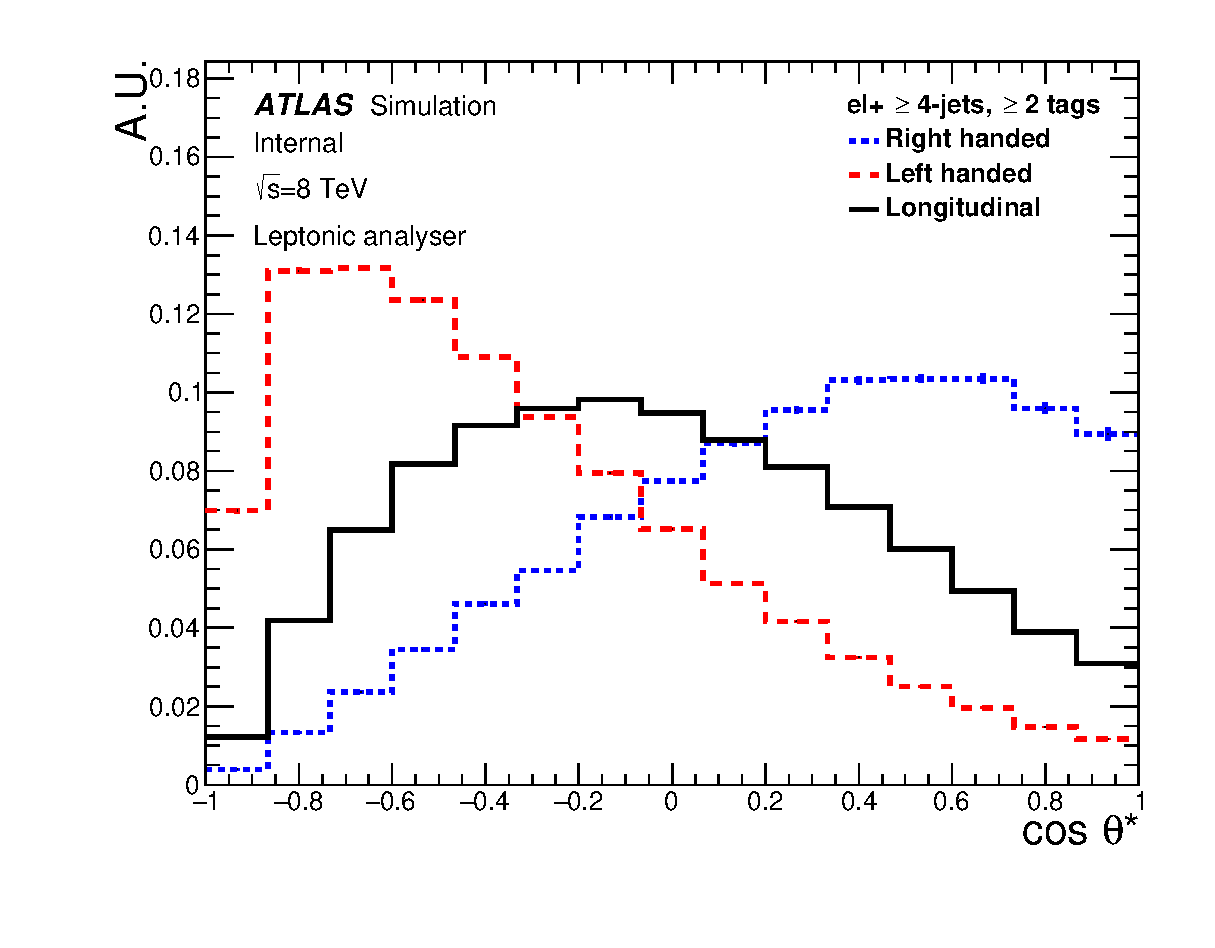
\includegraphics[height=58mm]{chapters/whel/figures/templatePlots/Leptonic/Signal_Templates_2incl_el_lep}
    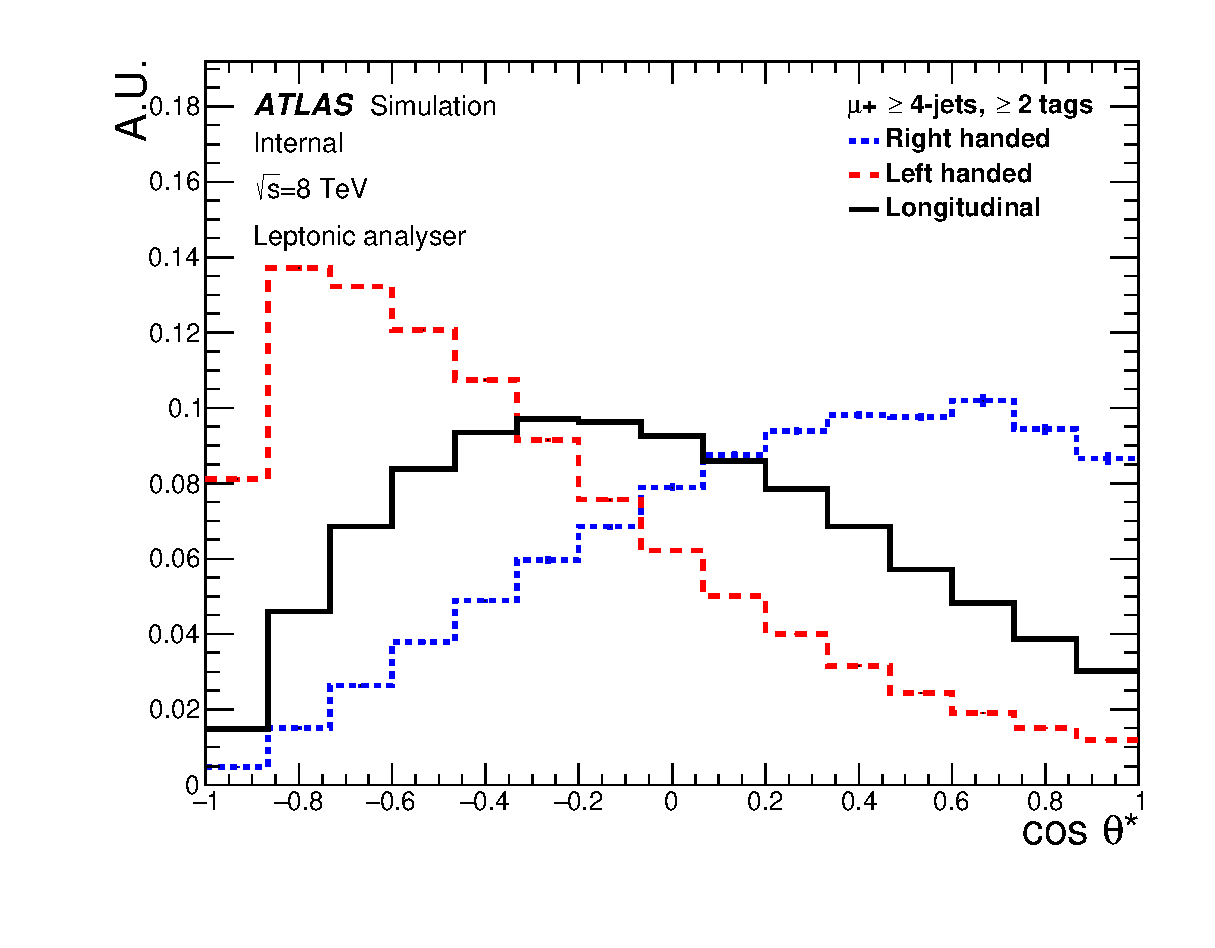
\includegraphics[height=58mm]{chapters/whel/figures/templatePlots/Leptonic/Signal_Templates_2incl_mu_lep}\\
    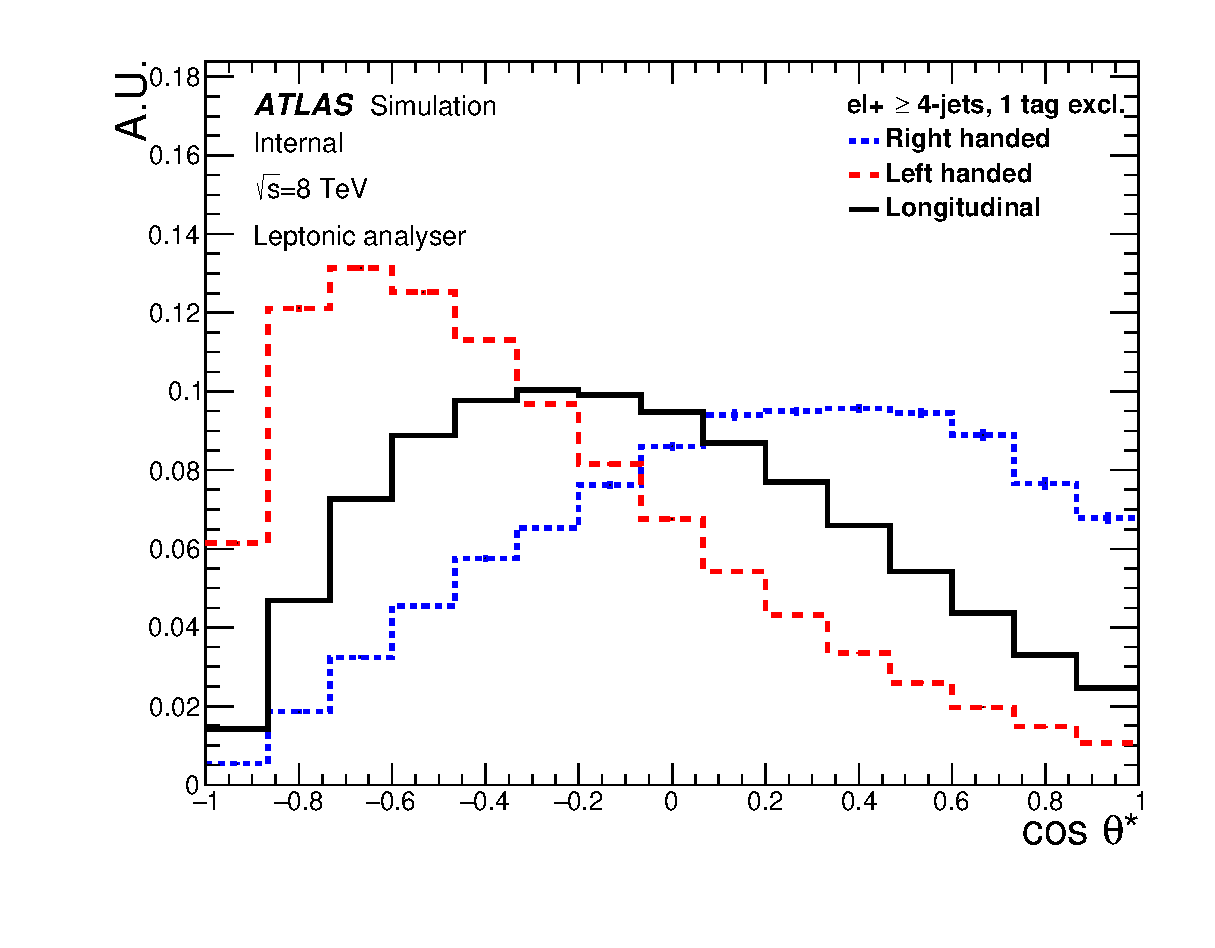
\includegraphics[height=58mm]{chapters/whel/figures/templatePlots/Leptonic/Signal_Templates_1excl_el_lep}
    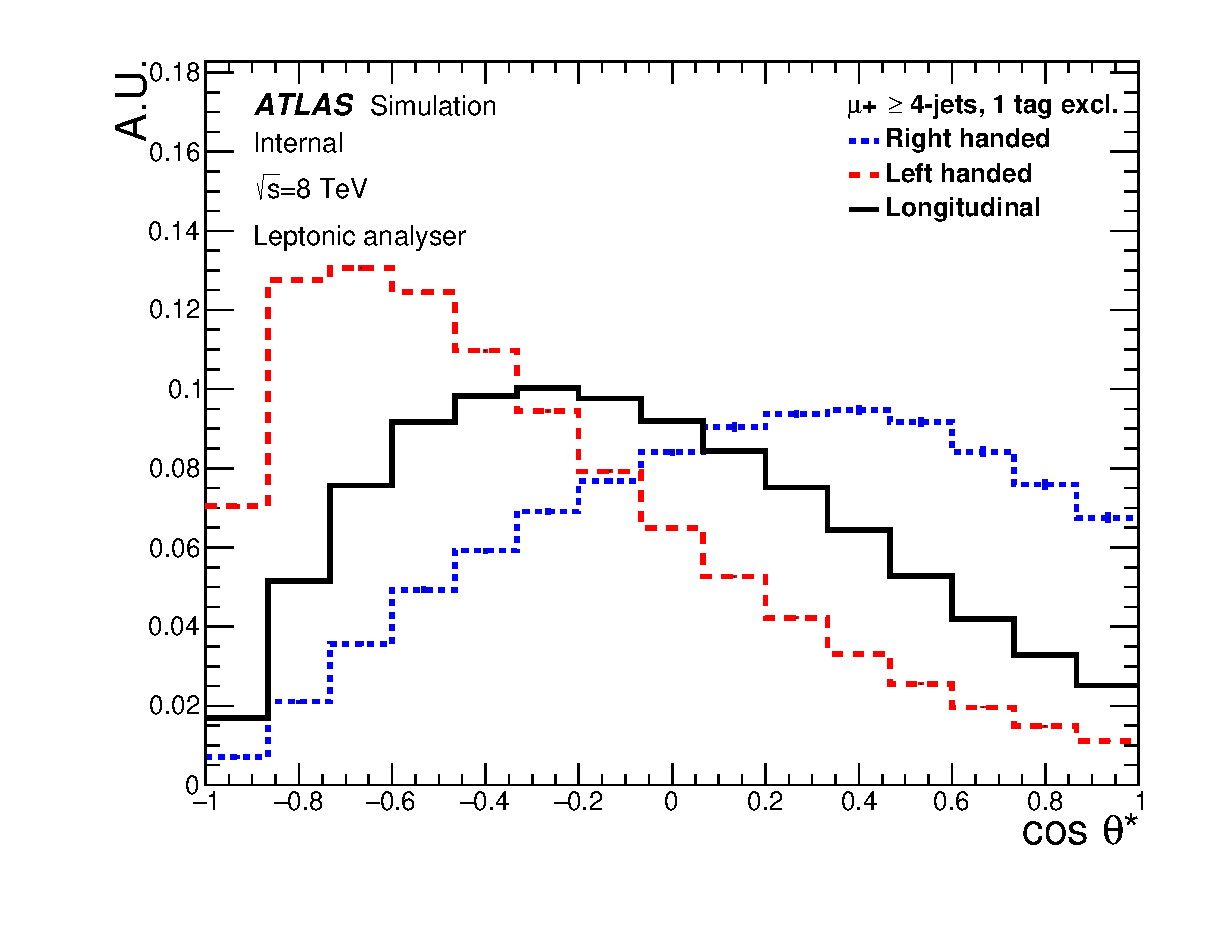
\includegraphics[height=58mm]{chapters/whel/figures/templatePlots/Leptonic/Signal_Templates_1excl_mu_lep}
    \caption{Reconstructed signal templates for $e$+jets channel (left) and $\mu$+jets channel (right) in the two inclusive \bt tag region (top) and one exclusive \bt tag region (bottom) for the leptonic angle.}
    \label{fig:Sig_temp_lep}
  \end{center}
\end{figure}


\begin{figure}[!hb]
  \begin{center}
    \includegraphics[height=58mm]{chapters/whel/figures/templatePlots/Hadronic/Signal_Templates_2incl_el_had}
    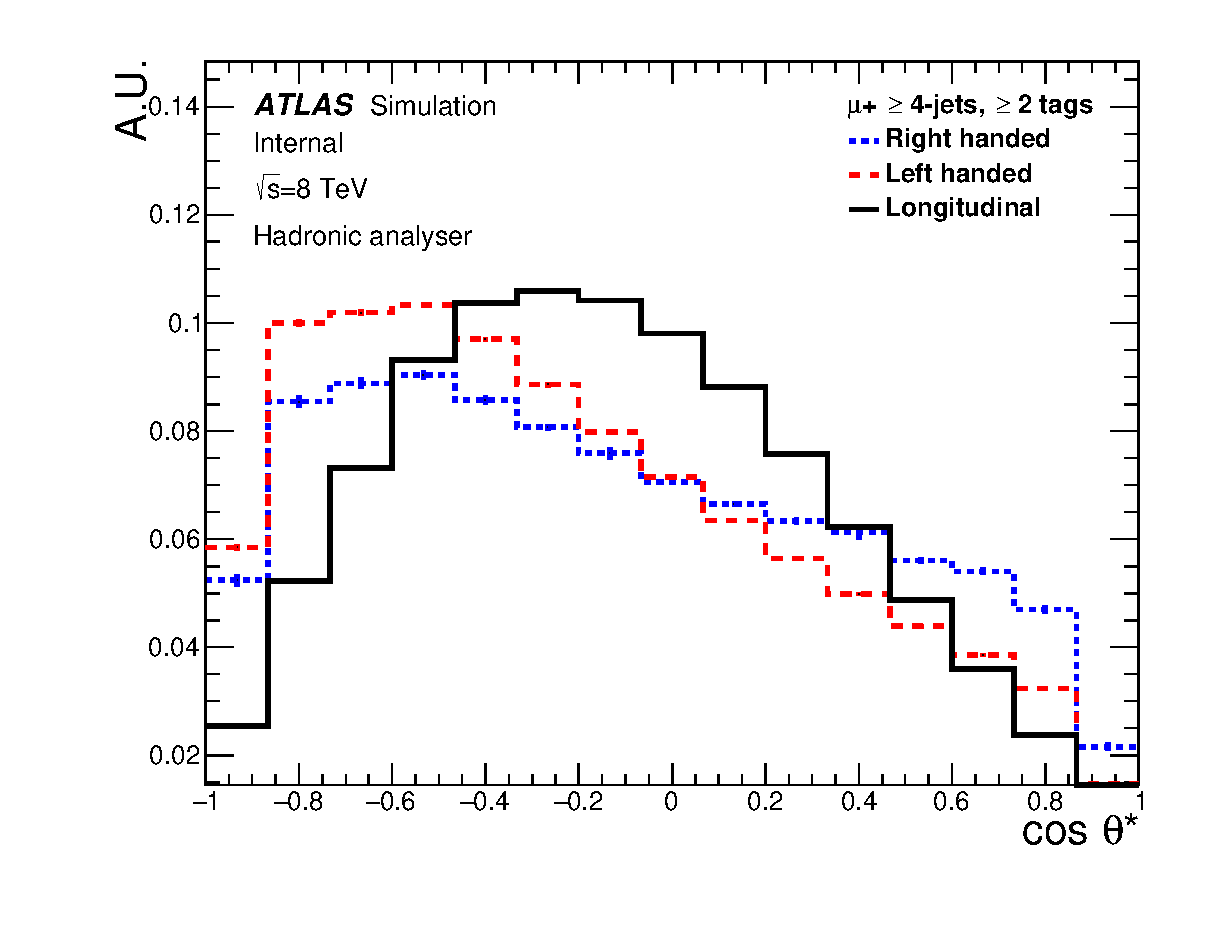
\includegraphics[height=58mm]{chapters/whel/figures/templatePlots/Hadronic/Signal_Templates_2incl_mu_had}\\
    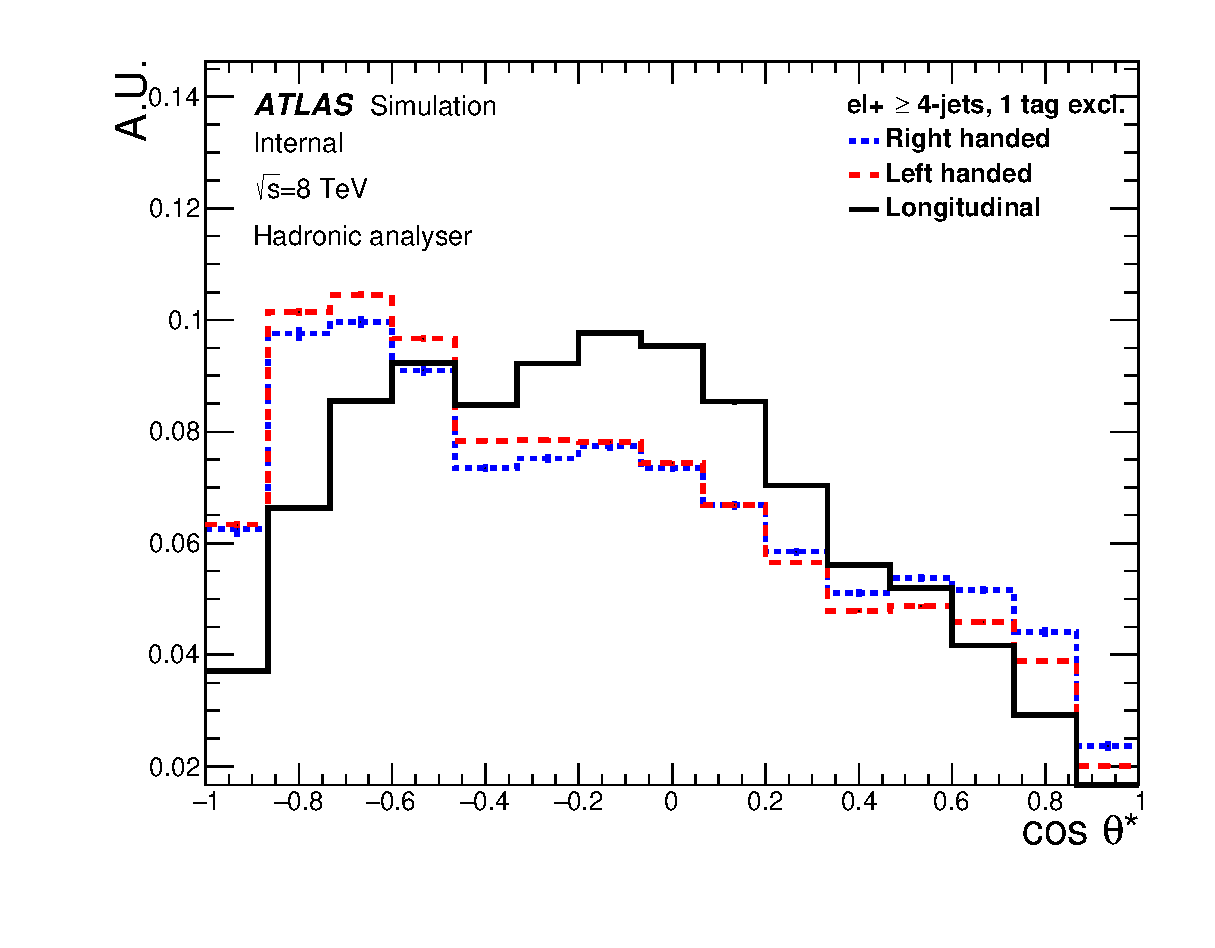
\includegraphics[height=58mm]{chapters/whel/figures/templatePlots/Hadronic/Signal_Templates_1excl_el_had}
    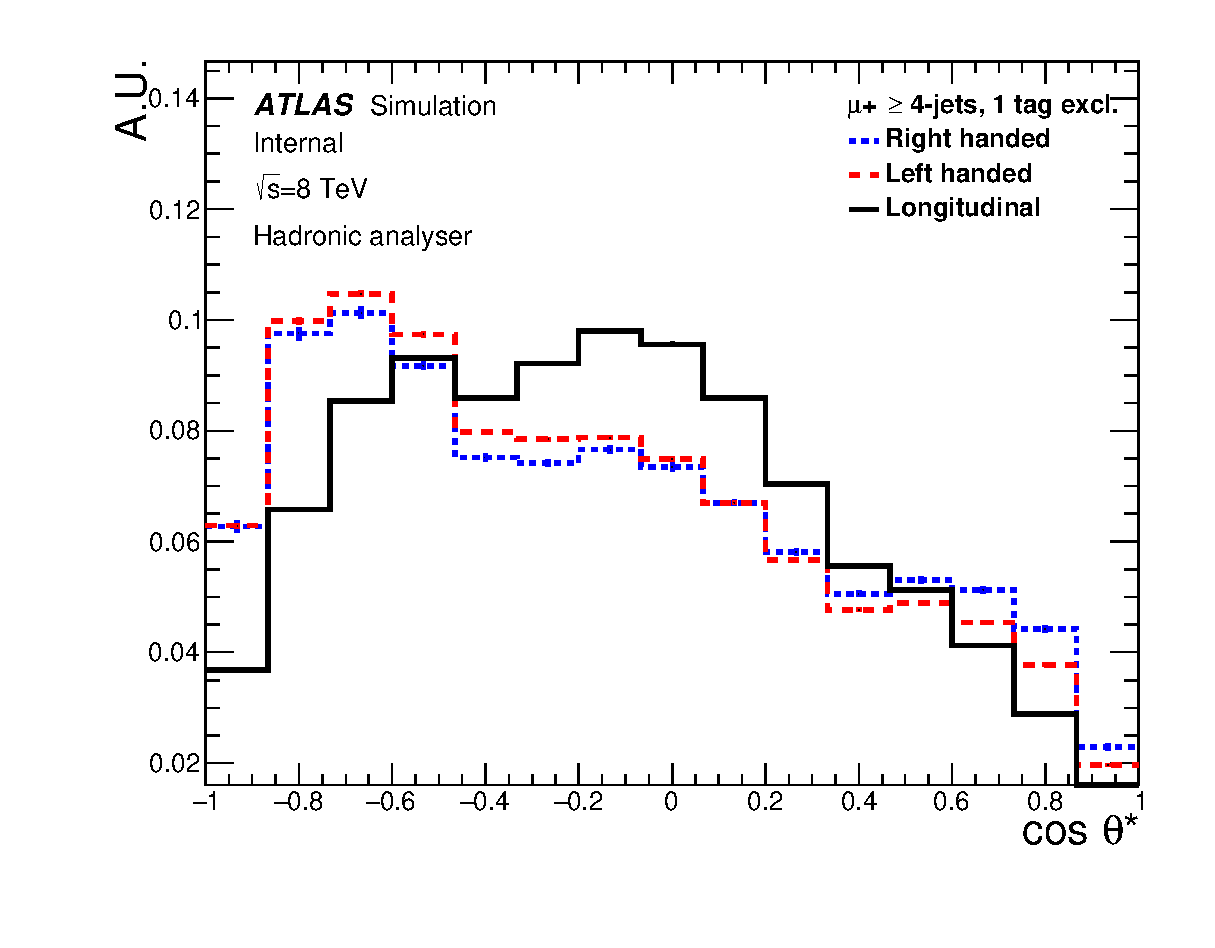
\includegraphics[height=58mm]{chapters/whel/figures/templatePlots/Hadronic/Signal_Templates_1excl_mu_had}
    \caption{Reconstructed signal templates for $e$+jets channel (left) and $\mu$+jets channel (right) in the two inclusive \bt tag region (top) and one exclusive \bt tag region (bottom) for the hadronic angle.}
    \label{fig:Sig_temp_had}
  \end{center}
\end{figure}

\begin{figure}[!hb]
  \begin{center}
    
    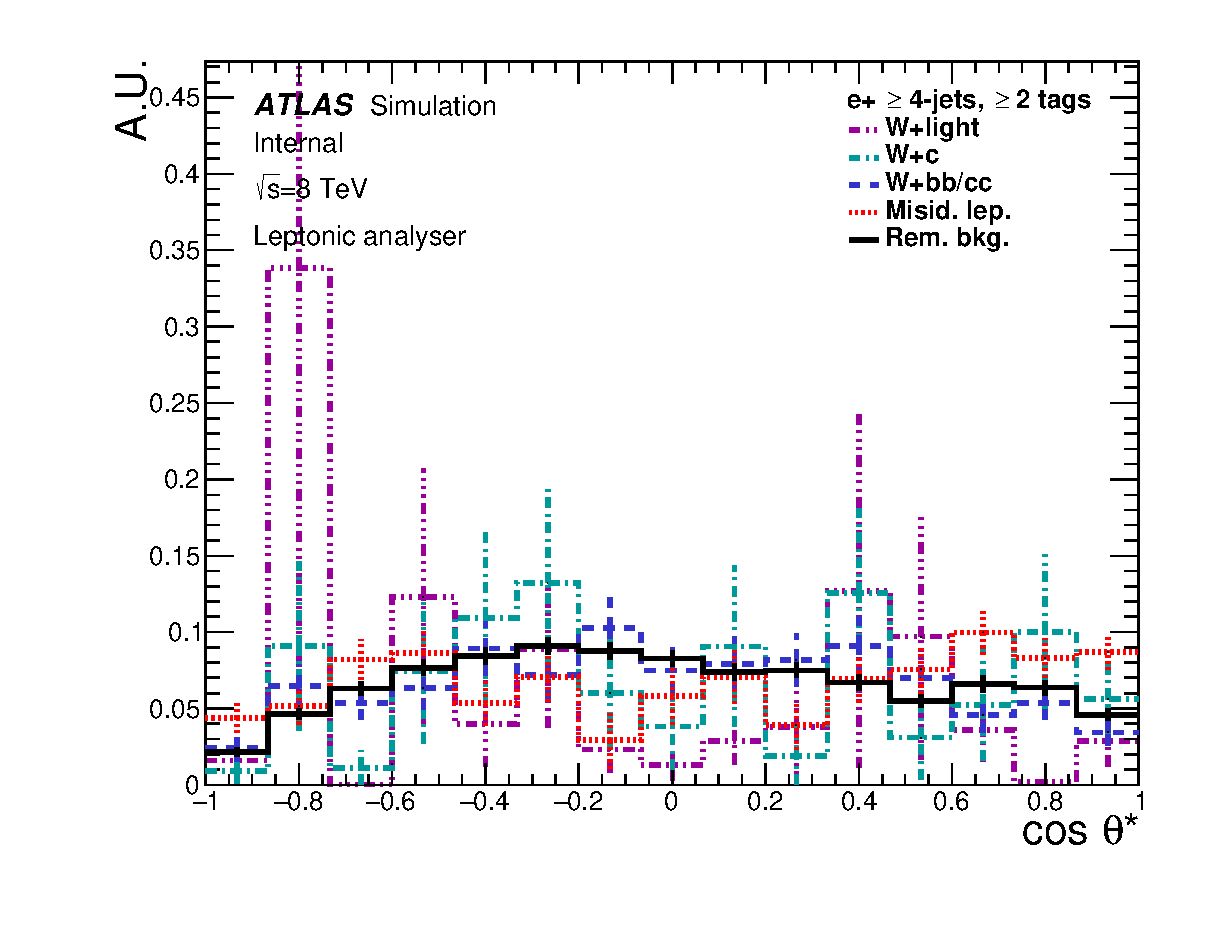
\includegraphics[height=58mm]{chapters/whel/figures/templatePlots/Leptonic/Background_Templates_2incl_el_lep}
    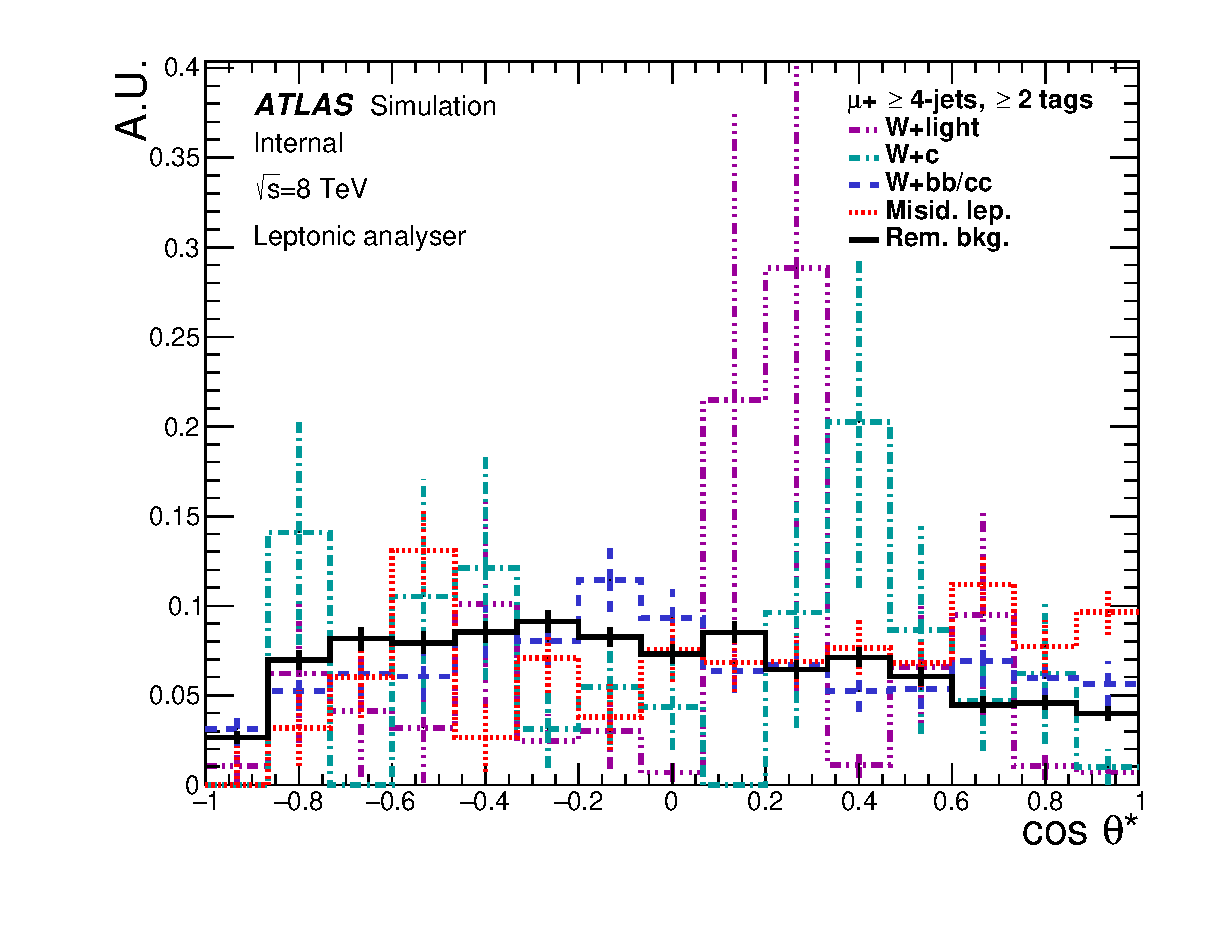
\includegraphics[height=58mm]{chapters/whel/figures/templatePlots/Leptonic/Background_Templates_2incl_mu_lep}\\
    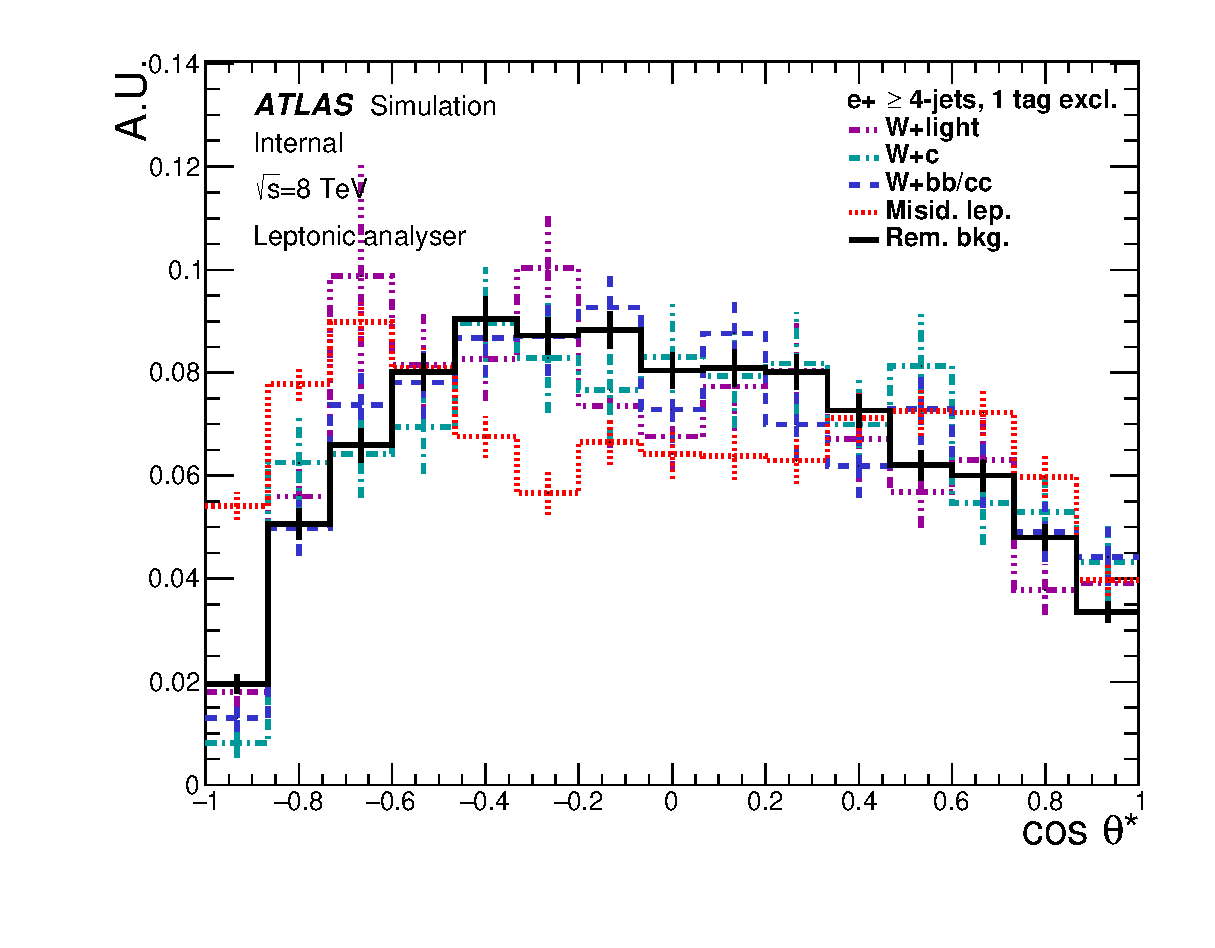
\includegraphics[height=58mm]{chapters/whel/figures/templatePlots/Leptonic/Background_Templates_1excl_el_lep}
    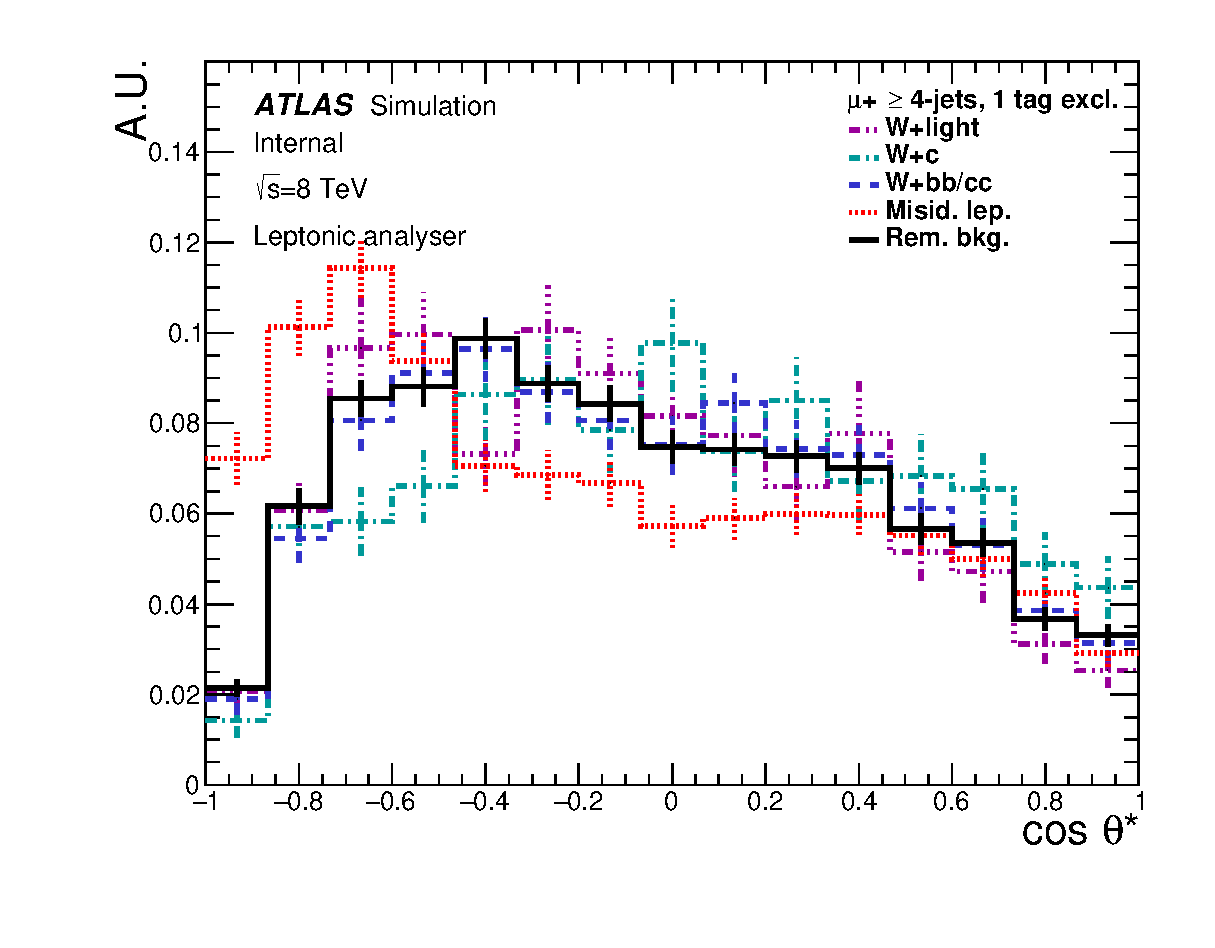
\includegraphics[height=58mm]{chapters/whel/figures/templatePlots/Leptonic/Background_Templates_1excl_mu_lep}
    \caption{Background templates for $e$+jets channel (left) and $\mu$+jets channel (right) in the two inclusive \bt tag region (top) and one exclusive \bt tag region (bottom) for the leptonic angle.}
    \label{fig:Bkg_temp_lep}
\end{center}
\end{figure}

\begin{figure}[!hb]
  \begin{center}
    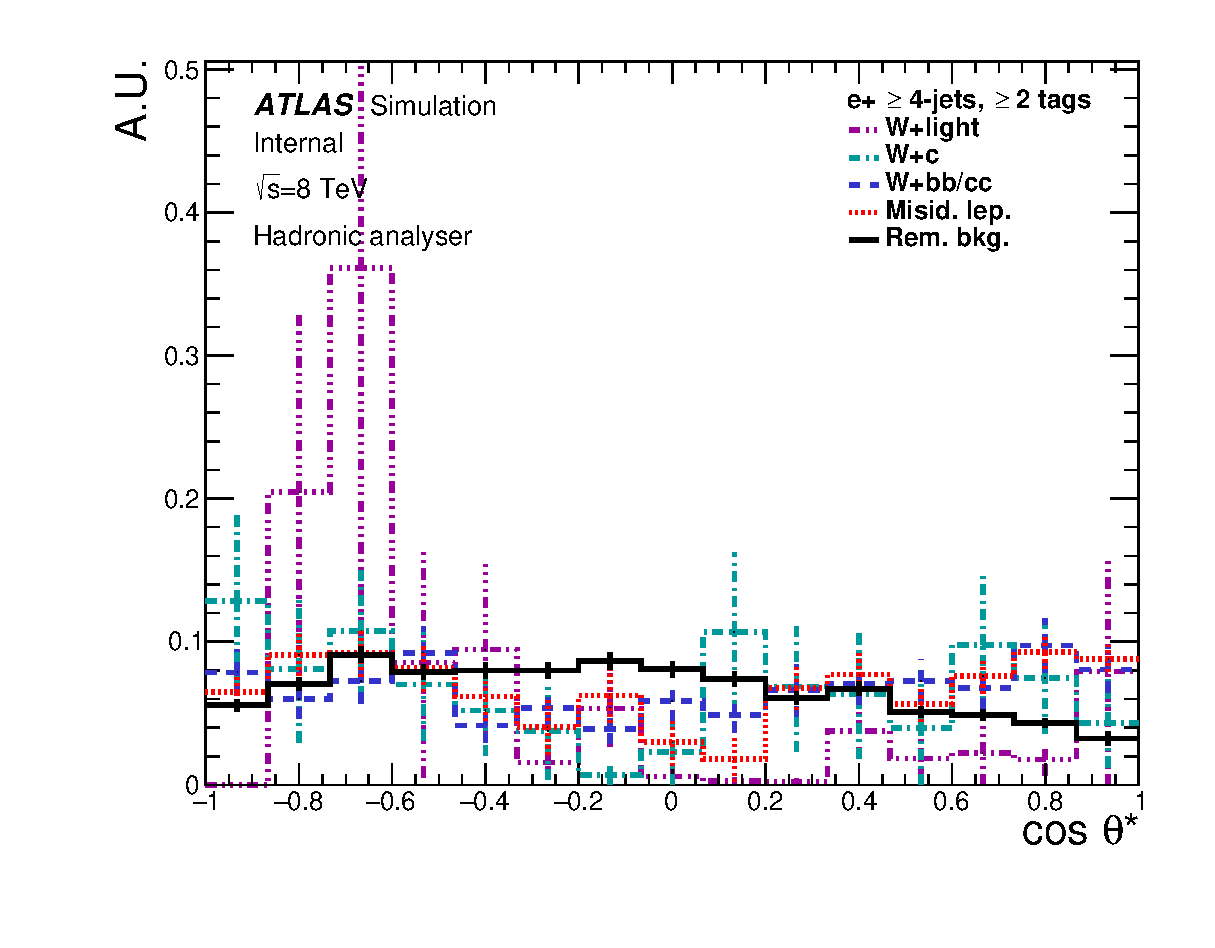
\includegraphics[height=58mm]{chapters/whel/figures/templatePlots/Hadronic/Background_Templates_2incl_el_had}
    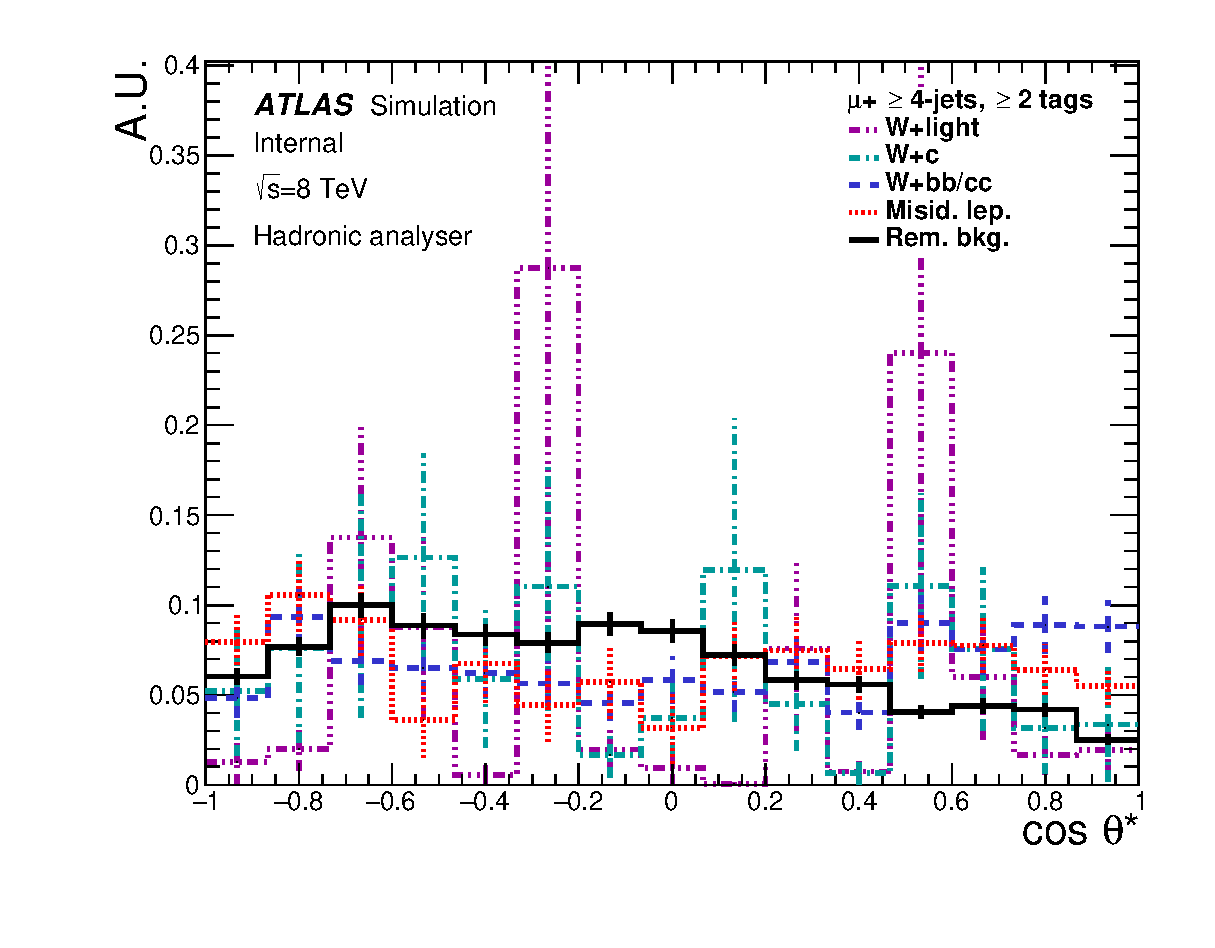
\includegraphics[height=58mm]{chapters/whel/figures/templatePlots/Hadronic/Background_Templates_2incl_mu_had}\\
    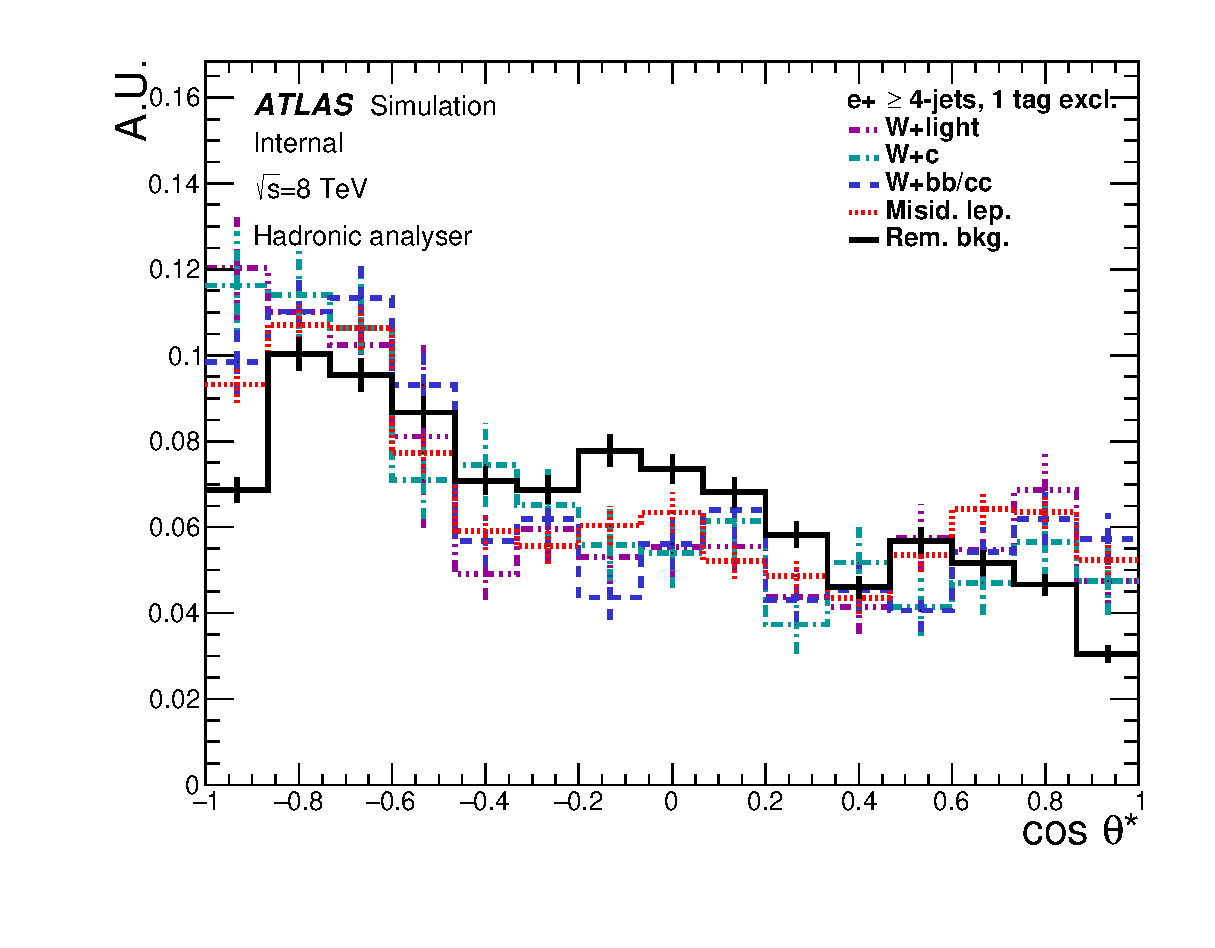
\includegraphics[height=58mm]{chapters/whel/figures/templatePlots/Hadronic/Background_Templates_1excl_el_had}
    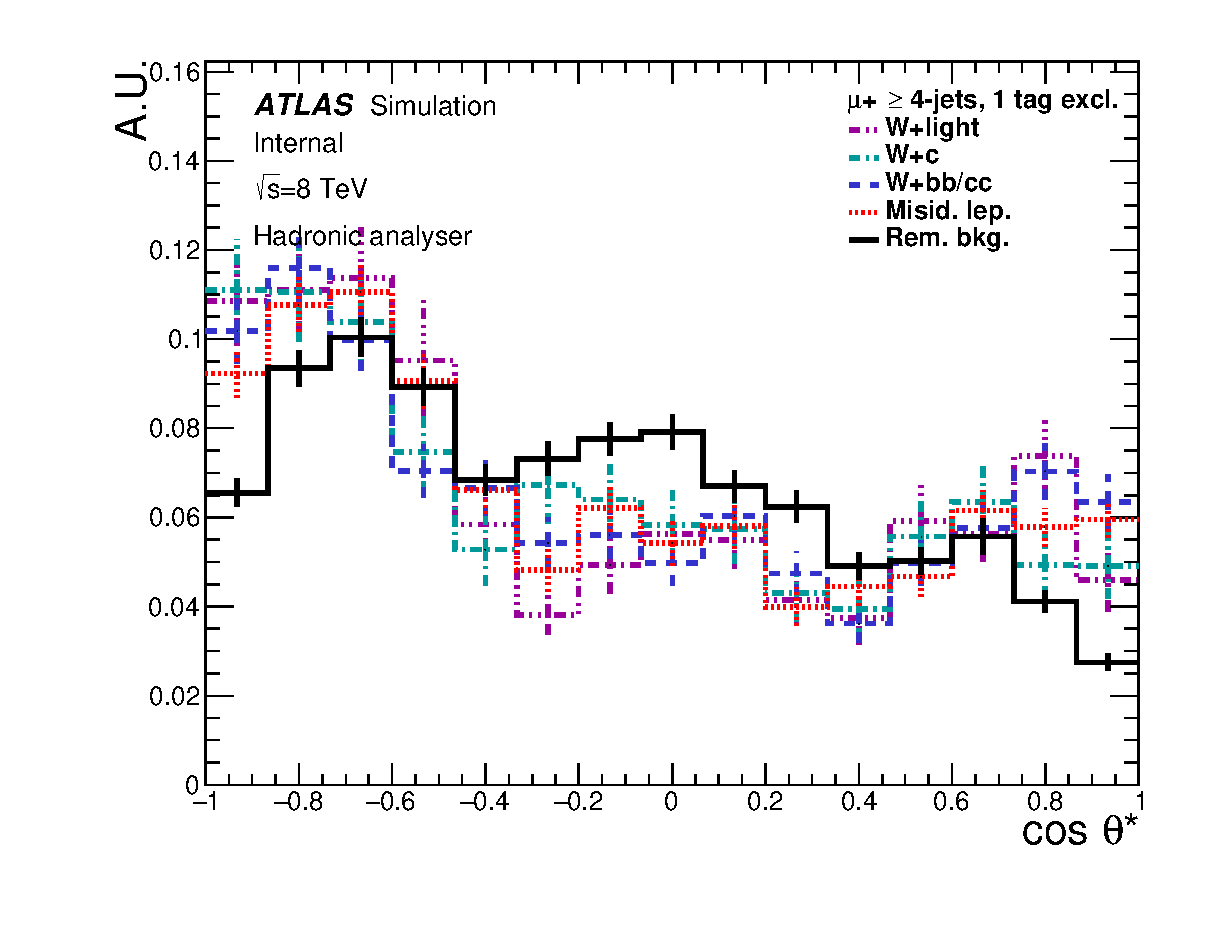
\includegraphics[height=58mm]{chapters/whel/figures/templatePlots/Hadronic/Background_Templates_1excl_mu_had}
    \caption{Background templates for $e$+jets channel (left) and $\mu$+jets channel (right) in  the two inclusive \bt tag region (top) and one exclusive \bt tag region (bottom) for the hadronic angle.}
    \label{fig:Bkg_temp_had}
  \end{center}
\end{figure}

 
\subsection{Likelihood Fit} 

A binned likelihood fit is performed using the signal and background templates mentioned above. The fit procedure is based on the ROOT {\sc Minuit} package \cite{James:310399},\cite{Brun:1997pa}. The normalizations of the backgrounds and the normalizations of each pure \ttbar helicity template are free parameters in the fit. The number of expected events in the fit corresponds to the sum of all template normalizations calculated and is calculated as:
\begin{equation}
n_{\textrm{exp, templ.}}= n_{\textrm{0, templ.}} + n_{\textrm{L, templ.}} +n_{\textrm{R, templ.}}+n_{\textrm{W+light}}+n_{\textrm{W+$c$}}+n_{\textrm{W+$bb/cc$}}+n_{\textrm{QCD}}+n_{\textrm{Rem.Bkg.}},   
\label{eq:nParams}
\end{equation}

to be compared in each bin to the data distribution from the likelihood fit:
\begin{equation}
{\mathscr{L}}=\prod\limits_{i=1}^{N_{\text{bins}}} \textrm{Poisson}(n_{\textrm{data},i}, n_{\textrm{exp},i}) \prod\limits_{j=1}^{N_{\text{bkg}}}\frac{1}{\sqrt{2\pi}\sigma_{\textrm{bkg.j}}}e^{\frac{-(n_{\textrm{bkg.j}}-\hat n_{\textrm{bkg.j}})^2}{2\sigma ^{2}_{\textrm{bkg.j}}}},
\label{eq:LHFit}
\end{equation}
where the background normalization uncertainties are constrained by Gaussian priors, and the $\sigma_{\textrm{bkg.j}}$ are the background normalization uncertainties for a given background. All free parameters in Eq. \ref{eq:nParams}, except for $n_{\text{QCD}}$, are common across all lepton/\bt tagged regions (e.g. the same $n_{\textrm{W+light}}$ parameter is common across all signal regions). The fake lepton normalization, $n_{\textrm{QCD}}$, is floated independently for electrons and muons and in different \bt tag regions. For the W +jets components, the normalization uncertainties are taken from the data-driven calibration factors~\cite{Juste:1647184}: 5\% for W +light jets, 25\% for W +c jets and 7\% for W +cc/bb jets. A relative uncertainty of 30\% is estimated for the matrix method QCD calculation\cite{MatrixMethod} and is used for the fake lepton contribution. An uncertainty of 16\% (17\%) is considered for the remaining background sources in the two inclusive \bt tag region (one exclusive + two inclusive \bt tag region) by adding the uncertainties on the theoretical cross sections of the single top quark, diboson and Z+jets components in quadrature with extra uncertainties accounting for additional jet reconstruction. For single top production, an uncertainty of 17\% is assumed, which takes into account the variation from the initial and final state radiation in t-channel samples and accounts for the single top +jets requirement in the 4 jets signal region. An overall normalization uncertainty of 48\% is applied to Z+jets and diboson contributions which takes into account 5\% uncertainty on the theoretical (N)NLO cross section and uncertainties to account for the extrapolation to high jet multiplicity (24\% per jet). A summary of all the free parameters in the fit and their uncertainties is given in Table \ref{tab:fitParams}. For most backgrounds, the normalizations are taken from simulation. Exceptionally, the normalization for misidentified leptons and $W$+jets events is taken from a data-driven method (see Section \ref{sec:backgroundAndSignalModelling} for details). These background normalizations and uncertainties are shown in Table \ref{tab:event_yield}.

The normalization for each helicity template is allowed to float unconstrained in the fit. Because the analysis is not equally sensitive to all helicity states, extraction of the production-level helicity fractions requires knowledge of the reconstruction efficiency per helicity state. These efficiencies, $\upepsilon_{i}^{\text{sel}}$, are calculated using the nominal \ttbar sample and are shown in Table \ref{tab:eff}. Given that the total \ttbar cross-section cancels in the calculation of the helicity fractions, the quantities $N_i$ are defined to translate the post-fit normalizations, $n_{\textrm{i, templ.}}$, into experimentally-independent quantities using these efficiencies. The relationship is given by
\begin{equation}
n_{\textrm{i, templ.}} = \upepsilon_{i}^{\text{sel}} \cdot N_{i}  \textrm{\quad for i= 0, L, R,}
\end{equation}

where, again, the $n_{\textrm{i, templ.}}$ are the parameters in the likelihood fit. Using $N_i$ allows the final helicity fractions to be expressed the simple ratio

\begin{equation}
F_{\text{i}}= \frac{N_{i}}{N_{0}+N_{L}+N_{R}}  \textrm{ \quad for i= 0, L, R.}
\label{eq:Frac}
\end{equation}

\begin{table}[]
\centering
\begin{tabular}{l|l}
\hline \hline
Fit Parameter & Relative Width of Gaussian Prior\\ \hline
n$_{\text{0}}$ & - \\
n$_{\text{L}}$ & - \\
n$_{\text{R}}$ & - \\
n$_{\text{\w+light}}$ & 0.05 \\
n$_{\text{\w+c}}$ & 0.25 \\
n$_{\text{\w+bb/cc}}$ & 0.07 \\
n$_{\text{QCD}}$ & 0.30 \\
n$_{\text{Rem. Bkg.}}$ & 0.16(0.17) in $\geqslant$ 2 \bt tags (1 \bt + $\geqslant$ 2 \bt tags) \\ \hline\hline
\end{tabular}
\caption{List of all free parameters in the bin-by-bin likelihood fit as well as the relative widths (width/normalization) of the Gaussian priors assumed in the fit with floating backgrounds.% The Rem. Bkg. category contains events passing selection from single top, $Z$+jets, and diboson Monte Carlo simulation. For the single top contribution, 17\% normalization uncertainty considered to cover the variation from the initial and final state radiationin t-channel samples and accounts for the single top +jets requirement in the 4 jets signal region. For $Z$+jets and diboson contributions, 4\% theory uncertainty is considered on the inclusive boson cross-section plus  24\% uncertainty per additional jet added in quadrature. For the \w+jets components, the uncertainties are taken from the data-driven calibration factors.
}
\label{tab:fitParams}
\end{table}

% OLD, REPLACED BY TABLE OF FIT PARAMETERS AND GAUSSIAN PRIORS
%\begin{table}[]
%\centering
%\begin{tabular}{l|l}
%\hline \hline
%Background & Normalization uncertainty \\ \hline
%W+jets & 0.48    \\
%QCD & 0.30     \\
%Rem. bkg. & 0.09(0.06) \\ \hline \hline
%\end{tabular}
%\caption{Background normalization uncertainty used in the fit with floating backgrounds. The background normalizations are allowed to float within these uncertainties in the fit with floating backgrounds. F%or the single top contribution, the theoretical cross section uncertainty is considered. For W+jets, Z+jets and diboson contributions, 4\% theory uncertainty is considered on the inclusive boson cross-secti%on plus  24\% uncertainty per additional jet added in quadrature. The uncertainty in parentheses in Rem. bkg. corresponds to muon channel. Other uncertainties applied in both $e$ and $\mu$ channels}
%\label{tab:bkgNormUnc}
%\end{table}

\subsection{Combining Fit Regions}
The combination of one exclusive and two inclusive \bt tag regions as well as the combination of $e$+jets and $\mu$+jets channels is studied. The channels are combined via a common likelihood fit; the signal templates for each of the respective helicity states are combined in an extended distribution with two/four/eight times the number of bins in the two/four/eight channel combination, while each background contribution is fit as described in the previous section. The selection efficiencies for the combined templates are adjusted accordingly. The summary of the pre-fit and post-fit yields in the combined electron + muon channel in two inclusive \bt tag region for leptonic analyzer and in one exclusive + two inclusive \bt region for the hadronic analyzer are shown in Tables \ref{tab:prepost_yields_lep2incl} and \ref{tab:prepost_yields_had_bTag} respectively.

\begin{table}
\centering 
\begin{tabular}{l|c|c|c|c}
  \hline\hline
  Parameter & Norm. unc. & Pre-fit & Post-fit & $\Delta \%$ \\ \hline\hline
  $t\bar{t}$ 		& - 	&  		& 2.87e+06 $\pm$ 44700	 &  \\ \hline
  W+light 			& 5\% 	& 68 	& 68 $\pm$ 3 	& 0.02 \\
  W+c 	 			& 25\% 	& 105 	& 105 $\pm$ 26 	& 0.3 \\
  W+bb/cc 			& 7\% 	& 1318 	& 1317 $\pm$ 92 & -0.08 \\ \hline
  QCD 2incl. (el) 	& 30\% 	& 447 	& 575 $\pm$ 117 & 28.6 \\
  QCD 2incl. (mu) 	& 30\% 	& 330  	& 285 $\pm$ 93  & -13.6 \\	\hline
  Rem. bkg. 		& 16\% 	& 2633	& 2629 $\pm$ 414 & -0.2 \\ \hline\hline

\end{tabular}
\caption{Pre-fit and post-fit yields comparison in the combined electron + muon channel in two inclusive \bt tag region for the leptonic analyzer.}
\label{tab:prepost_yields_lep2incl}
\end{table}

\begin{table}
\centering 
\begin{tabular}{l|c|c|c|c}
  \hline\hline
  Parameter & Norm. unc. & Pre-fit & Post-fit & $\Delta \%$ \\ \hline\hline
  $t\bar{t}$ 		& - &  & 2.90e+06 $\pm$ 94400	 &  \\ \hline
  W+light 			& 5\% 	& 1430 	& 1424 $\pm$ 71  & -0.4\\
  W+c 	 			& 25\% 	& 2756 	& 2070 $\pm$ 577 & -24.9  \\
  W+bb/cc 			& 7\% 	& 7565 	& 7298 $\pm$ 495 & -3.5 \\ \hline
  QCD 1excl. (el) 	& 30\% 	& 2272 	& 1431 $\pm$ 348 & -37    \\
  QCD 1excl. (mu) 	& 30\% 	& 447 	& 620 $\pm$ 111  & 38.7   \\
  QCD 2incl. (el) 	& 30\% 	& 1746 	& 1379 $\pm$ 340 & -21   \\
  QCD 2incl. (mu) 	& 30\% 	& 323  	& 283 $\pm$ 92   & -12.3 \\	\hline
  Rem. bkg. 		& 17\% 	& 9191 	& 6019 $\pm$ 1290 & -34.5  \\ \hline\hline

\end{tabular}
\caption{Pre-fit and post-fit yields comparison in the combined electron + muon channel in one exclusive + two inclusive \bt tag region for the hadronic analyzer.}
\label{tab:prepost_yields_had_bTag}
\end{table}

\subsection{Correlations Between Leptonic and Hadronic Measurements}
Since there are two simultaneous measurements being performed per event (the angles from leptonically and hadronically decaying \w bosons), the correlation between the two angles needs to be quantified. Even though they are, in principle, uncorrelated as the decays themselves are independent, a non-zero correlation could be introduced through the reconstruction. In the case of non-negligible correlation, it would be incorrect to evaluate the uncertainties in the different channels independently, and the correlation would need to be correctly accounted for. In the case of negligible correlation, the two channels can be treated and evaluated fully independently.

To estimate the correlation, two-dimensional plots (one angle per axis) are produced and the correlation factor (=-1 for perfect anti-correlation, = +1 for perfect correlation, = 0 for 100\% uncorrelated) calculated. The plots are shown in Figure \ref{fig:twoD_correlation}. The correlation factor is evaluated for all events with at least two \bt tags passing the nominal selection as well as for the subset events with log(LH)$>-48$ (discussed in Section \ref{sec:hadronicOptimization} for optimizing hadronic sensitivity).

\begin{figure}[htbp]
  \begin{center}
    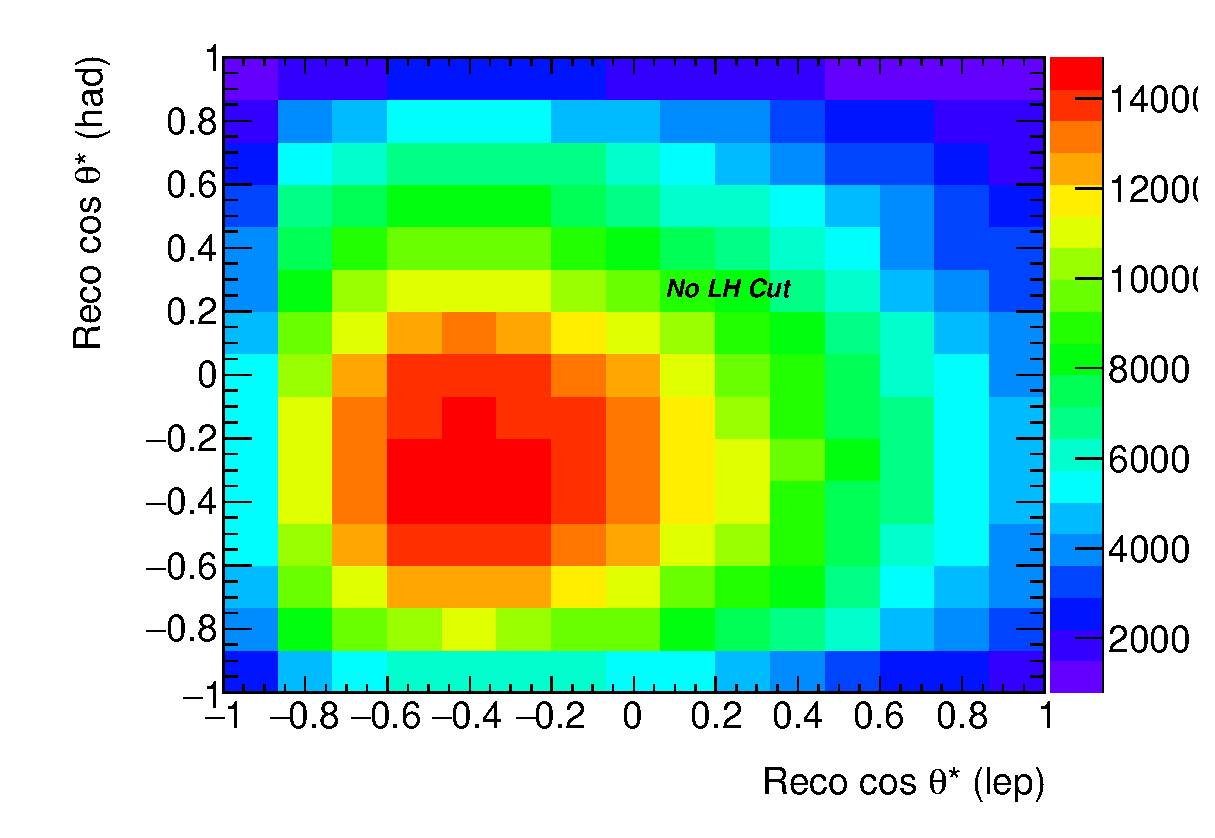
\includegraphics[height=50mm]{chapters/whel/figures/twoDimCorrelation/costheta_2D_noLH}
    \includegraphics[height=50mm]{chapters/whel/figures/twoDimCorrelation/costheta_2D_withLH}
    \caption{Two-dimensional distributions of the reconstructed leptonic and hadronic cos $\theta^*$ in all events with two or more \bt tags passing the nominal selection (left) and passing the nominal selection plus the cut LH $>-48$ to optimize the sensitivity of the hadronic analyzer.}
    \label{fig:twoD_correlation}
  \end{center}
\end{figure}

The correlation factor is calculated to be -0.0038 for the nominal selection and -0.0029 when imposing the LH cut. The correlation is considered to be negligible in both cases, and the measurements are considered to be independent for the remainder of this analysis.

\subsection{Evaluation of Systematic and Expected Statistical Uncertainties}
\label{sec:statisticalUnc}
 Ensemble tests are performed for the estimation of systematic and expected statistical uncertainties. Pseudo-data distributions are produced using MC simulation and scaled to the actual data statistics. Ensembles (pseudo-experiments) are obtained by fluctuating each bin of the pseudo-data distribution according to Poisson statistics. For the template fit, 5,000 pseudo-experiments are generated. The mean values of $N_{0}$ , $N_{L}$ and $N_{R}$ are used to calculate the specific W-helicity fractions for each pseudo-data distribution. The differences between the fractions obtained from the nominal distribution and the fractions obtained from each systematic variation are considered. For systematics with up and down variations, the calculated systematic shifts are added in quadrature. For one-sided sources of systematic uncertainty (e.g. jet energy resolution, signal modeling systematics), the single variation is symmetrized and taken as both the up and down variations. All contributions summed in quadrature.
 
 The expected statistical uncertainties are obtained from fits to the pseudo-data distributions, where {\sc Minuit} provides the fitted number of events and the corresponding statistical uncertainties. Since the helicity fractions are obtained from the fitted number of events, the error propagation is considered accordingly. Table \ref{tab:statUnc_fix_LH_comparison} summarizes the statistical uncertainty expectation obtained in each channel from ensemble test fits. The normalization of the background contributions were kept fixed during these tests in order to estimate the absolute statistical uncertainty. %In each \bt tag region (1 excl. and 2incl. \bt tag), the $e$+jets and $\mu$+jets channels are combined. The one exclusive and two inclusive \bt tag regions are also combined for the electron and muon channel separately. The four-channel combination includes both leptons in both \bt tag regions. As expected, all combinations yield better statistical sensitivities than any individual region while the four-channel combination provides the best expected statistical uncertainties for all helicity fractions.
 In each \w boson decay (leptonic and hadronic), the $e$+jets and $\mu$+jets channels are combined. The combined sensitivities are high as expected from the increase in statistics. The eight-channel combination including both leptonic and hadronic sides, provides the lowest expected statistical uncertainty. %The corresponding helicity fractions distributions are presented in Appendix ~\ref{app:expectedStatUnc}.

As seen in table \ref{tab:statUnc_fix_LH_comparison}, the expected statistical sensitivities are worse for the helicity fractions fit from the hadronic side than those fits from the leptonic one. This is a reflection of the imperfect identification of the up and down type jets from the decay of the hadronic \w boson which results in a lower discrimination between the pure, re-weighted templates. The sensitivity of the hadronic extraction is improved by requiring the log likelihood of the leading permutation be greater than -48. This optimization is discussed in Section \ref{sec:hadronicOptimization}.

Five thousand pseudo-experiments are performed to evaluate the sensitivity of the leptonic channel both with and without the likelihood cut derived from the hadronic optimization. The sensitivity of the eight-channel combination measurement is also evaluated when the likelihood cut was applied to both channels and when it was applied to the hadronic channel alone. The results are summarized in same table and show negligible difference. To simplify the combination and of the leptonic and hadronic measurements, the same likelihood cut is imposed for both the leptonic and hadronic measurements. Using identical phase spaces has the additional benefit of allowing the background templates to be treated as correlated quantities in the leptonic+hadronic combination fit.  

\begin{table}[]
\centering
\begin{tabular}{c|c|c|c|c}
\hline \hline
Selection eff.   & $e$+jets (lep) & $\mu$+jets (lep)  & $e$+jets (had) & $\mu$+jets (had) \\ 
\hline \hline
\multicolumn{5}{c}{1 Exclusive \bt tag}\\
\hline
$\upepsilon_{0}$ & 0.014   & 0.017 &   0.014   & 0.016     \\
$\upepsilon_{L}$ & 0.010   & 0.013 &   0.012   & 0.014    \\
$\upepsilon_{R}$ & 0.015   & 0.017 &   0.012   & 0.014    \\ 

\hline
\multicolumn{5}{c}{2 Inclusive \bt tags}\\
\hline
%Selection eff.   & el+jets (lep) & $\mu$+jets (lep)  & el+jets (had) & $\mu$+jets (had) \\ \hline
$\upepsilon_{0}$ &   0.014   &   0.017   &   0.013   & 0.016     \\
$\upepsilon_{L}$ &   0.010   &   0.012   &   0.012   & 0.014    \\
$\upepsilon_{R}$ &   0.016   &   0.018   &   0.012   & 0.014    \\ \hline \hline
\end{tabular}
\caption{Selection efficiencies in the 1 exclusive and 2 inclusive \bt tag regions for both the leptonic and hadronic templates in the $e$+jets and $\mu$+jets channel.} %The efficiencies are lower in the hadronic channel due to the cut on log likelihood and comparable between \bt tag regions as the \ttbar yields are similar.}

\label{tab:eff}
\end{table}

%\begin{table}[]
%\centering
%\caption{Absolute statistical uncertainty expectations of the helicity fractions fitted using the leptonic angle.}
   %%\label{my-label}
   %%\begin{tabular}{|l|l|l|l|l|}
%\begin{tabular}{c|c|c|c|c}
%\hline \hline
%Channel                   &                & 1 \bt tag excl. & 2 \bt tag incl. & Combined \\ \hline \hline
%\multirow{3}{*}{$e$+jets}  & $\sigma_{ \text{F}_{0}}$ & 0.0241         & 0.0157         & 0.0134    \\ 
                          %& $\sigma_{ \text{F}_{L}}$ & 0.0145         & 0.0101        & 0.0085  \\  
                          %& $\sigma_{ \text{F}_{R}}$ & 0.0117         & 0.0072         & 0.0062    \\ \hline
%\multirow{3}{*}{$\mu$+jets} & $\sigma_{ \text{F}_{0}}$ & 0.0212         & 0.0140         & 0.0121    \\ 
                          %& $\sigma_{ \text{F}_{L}}$ & 0.0127         & 0.0089         & 0.0075   \\  
                          %& $\sigma_{ \text{F}_{R}}$ & 0.0103         & 0.0066        & 0.0057  \\ \hline
%\multirow{3}{*}{Combined} & $\sigma_{ \text{F}_{0}}$ & 0.0161         & 0.0105         & 0.0089    \\  
                          %& $\sigma_{ \text{F}_{L}}$ & 0.0097         & 0.0067         & 0.0056   \\ 
                          %& $\sigma_{ \text{F}_{R}}$ & 0.0075         & 0.0048         & 0.0042   \\ \hline \hline
%\hline
%\end{tabular}
%\label{tab:statUnc_lep}
%\end{table}

%\begin{table}[]
%\centering
%\caption{Absolute statistical uncertainty expectations of the helicity fractions fitted using the hadronic angle when the leading log likelihood is required to be $>-48$.}
%\label{my-label}
%%\begin{tabular}{|l|l|l|l|l|}
%\begin{tabular}{c|c|c|c|c}
%\hline
%Channel                   &                & 1 \bt tag excl. & 2 \bt tag incl. & Combined \\ \hline \hline
%\multirow{3}{*}{$e$+jets}  & $\sigma_{ \text{F}_{0}}$ & 0.0311        & 0.0245        & 0.0183    \\ 
                          %& $\sigma_{ \text{F}_{L}}$ & 0.1283        & 0.0407        & 0.0390  \\  
                          %& $\sigma_{ \text{F}_{R}}$ & 0.1179        & 0.0409        & 0.0371    \\ \hline
%\multirow{3}{*}{$\mu$+jets} & $\sigma_{ \text{F}_{0}}$ & 0.0279        & 0.0203        & 0.0160\\ 
                          %& $\sigma_{ \text{F}_{L}}$ & 0.1003        & 0.0360        & 0.0331   \\  
                          %& $\sigma_{ \text{F}_{R}}$ & 0.0906        & 0.0360        & 0.0324 \\ \hline
%\multirow{3}{*}{Combined} & $\sigma_{ \text{F}_{0}}$ & 0.0203        & 0.0155        & 0.0121    \\  
                          %& $\sigma_{ \text{F}_{L}}$ & 0.0785        & 0.0264        & 0.0251   \\ 
                          %& $\sigma_{ \text{F}_{R}}$ & 0.0712        & 0.0260        & 0.0243   \\ \hline \hline 
%\hline
%\end{tabular}
%\label{tab:statUnc_had}
%\end{table}

%%%%%%%%% new table for 110404 sample and only 2incl b tag --- fixed bkg
\begin{table}[]
\centering
   %\label{my-label}
   %\begin{tabular}{|l|l|l|l|l|}
\begin{tabular}{c|c|c|c}
\hline \hline
Cut                       &                                      & 2incl. \bt tag & 1excl+2incl \bt tag \\ \hline \hline
\multicolumn{4}{c}{Leptonic side}\\ \hline
\multirow{3}{*}{no LH cut}  & $\sigma_{ \text{F}_{0}}$           & 0.010 $\pm$ 1.0\%  & 0.009 $\pm$ 1.0\%  \\ 
                          & $\sigma_{ \text{F}_{L}}$             & 0.006 $\pm$ 1.0\% &  0.005 $\pm$ 1.0\% \\  
                          & $\sigma_{ \text{F}_{R}}$             & 0.005 $\pm$ 1.0\% &  0.004 $\pm$ 1.0\% \\ \hline
\multirow{3}{*}{LH \textgreater -48} & $\sigma_{ \text{F}_{0}}$  & 0.012 $\pm$ 1.3\% &  0.010 $\pm$ 1.1\%   \\ 
                          & $\sigma_{ \text{F}_{L}}$             & 0.008 $\pm$ 1.3\% &  0.006 $\pm$ 1.0\%  \\  
                          & $\sigma_{ \text{F}_{R}}$             & 0.006 $\pm$ 1.3\% &  0.004 $\pm$ 1.1\%  \\ \hline \hline
\multicolumn{4}{c}{Hadronic side}\\ \hline
\multirow{3}{*}{LH \textgreater -48} & $\sigma_{ \text{F}_{0}}$  & 0.012 $\pm$ 1.0\% &  0.010 $\pm$ 1.0\%   \\ 
                          & $\sigma_{ \text{F}_{L}}$             & 0.022 $\pm$ 1.1\% &  0.021 $\pm$ 1.0\%   \\  
                          & $\sigma_{ \text{F}_{R}}$             & 0.022 $\pm$ 1.0\% &  0.021 $\pm$ 1.1\%   \\ \hline \hline
\multicolumn{4}{c}{Leptonic + hadronic combination}\\ \hline
\multirow{3}{*}{LH \textgreater -48 in hadronic side} & $\sigma_{ \text{F}_{0}}$ & 0.008 $\pm$ 1.0\% & 0.007 $\pm$ 1.1\% \\ 
                          							  & $\sigma_{ \text{F}_{L}}$ & 0.005 $\pm$ 1.0\% & 0.004 $\pm$ 1.1\% \\  
                          							  & $\sigma_{ \text{F}_{R}}$ & 0.004 $\pm$ 1.0\% & 0.003 $\pm$ 1.0\% \\ \hline
\multirow{2}{*}{LH \textgreater -48 in both sides} 	  & $\sigma_{ \text{F}_{0}}$ & 0.008 $\pm$ 1.0\% & 0.007 $\pm$ 1.0\%  \\ 
                          							  & $\sigma_{ \text{F}_{L}}$ & 0.006 $\pm$ 1.0\% & 0.005 $\pm$ 1.0\%  \\  
                         							  & $\sigma_{ \text{F}_{R}}$ & 0.004 $\pm$ 1.0\% & 0.004 $\pm$ 1.0\%  \\ \hline \hline

\hline
\end{tabular}
\caption{Absolute statistical uncertainty expectations of the helicity fractions fitted using the leptonic side, hadronic side and combined in 2 inclusive \bt tag and the combined 1excl. + 2incl. \bt tag. The requirement of the leading log likelihood to be $>-48$ is applied to the hadronic analyzer and also studied for the leptonic analyzer. The combined leptonic + hadronic sides is also presented for both cut options. The background normalization uncertainties kept fixed in the fit. The relative errors presenting the error in obtaining the Gaussian width  of each helicity fraction distribution.  %The final column presents the size of the combined uncertainty for each row with respect the SM-predicted value for each helicity fraction.
}
\label{tab:statUnc_fix_LH_comparison}
\end{table}

%The background normalization could be treated either as fixed to their Monte Carlo predictions in the fit or be allowed to float within their theoretical uncertainties according to Gaussian prior . In the later scenario, the width of the obtained helicity fraction distributions of fitting five thousand pseudo-experiments presents the expected statistical + background normalization uncertainties. On the other hand, in the former scenario, the width of the helicity distributions presents the absolute expected statistical uncertainty as mentioned before. The results of this comparison are summarised in table \ref{tab:statUnc_floatVSfix}. In general, the test is showing stability against the different background normalization treatments in the fit with respect to the expected statistical (statistical + background normalization) uncertainties for fixed (floating) treatments. Due to the smaller systematic uncertainties, the floating background normalization treatment is chosen as the default method in this analysis.

Table \ref{tab:DataFit_floatVSfix} compares the measured helicity fractions obtained from fit to data when the background normalizations are fixed to their Monte Carlo predictions and when they are allowed to float within their theoretical uncertainties according their associated Gaussian priors. Since the floating background normalization treatment takes the background normalization uncertainties into account, the systematic uncertainties due to background normalization uncertainties are evaluated individually in the fixed background configuration. The up (down) variation of each background is obtained by increasing (decreasing) the corresponding normalization by the upper (lower) normalization uncertainty while keeping fixing the other backgrounds normalizations to their nominal values. The total background normalization uncertainty is the quadrature sum of all components after symmetrization. The helicity fractions obtained using the fixed background configuration are consistent with the results obtained by using the floating background normalization configuration. %The corresponding tables are provided in Appendix \ref{app:bkgNormSyst}.


%In addition, the statistical correlation between \fo, \fl and \fr is provided in Appendix \ref{app:fractionCorrelations}.

\begin{comment}
\begin{table}[]
\centering
   %\label{my-label}
   %\begin{tabular}{|l|l|l|l|l|}
\begin{tabular}{c|c|c|c}
\hline \hline
Background norm. unc. mode   &  & 2incl. \bt tag & 1excl+2incl \bt tag \\ \hline \hline
\multicolumn{4}{c}{Leptonic side}\\ \hline
\multirow{3}{*}{Fixed}  & $\sigma_{ \text{F}_{0}}$       & 0.012 $\pm$ 1.0\% &  0.010 $\pm$ 1.1\%   \\ 
                          & $\sigma_{ \text{F}_{L}}$     & 0.008 $\pm$ 1.0\% &  0.006 $\pm$ 1.0\%   \\  
                          & $\sigma_{ \text{F}_{R}}$     & 0.006 $\pm$ 1.0\% &  0.004 $\pm$ 1.1\%   \\ \hline
\multirow{3}{*}{Floating} & $\sigma_{ \text{F}_{0}}$  	 & 0.012 $\pm$ 1.0\% &  0.010 $\pm$ 1.0\%   \\ 
                          & $\sigma_{ \text{F}_{L}}$     & 0.008 $\pm$ 1.0\% &  0.006 $\pm$ 1.0\%  \\  
                          & $\sigma_{ \text{F}_{R}}$     & 0.006 $\pm$ 1.0\% &  0.005 $\pm$ 1.0\%  \\ \hline \hline
\multicolumn{4}{c}{Hadronic side}\\ \hline
\multirow{3}{*}{Fixed}    & $\sigma_{ \text{F}_{0}}$  	& 0.012 $\pm$ 1.0\% &  0.010 $\pm$ 1.0\%   \\ 
                          & $\sigma_{ \text{F}_{L}}$    & 0.022 $\pm$ 1.1\% &  0.021 $\pm$ 1.0\%   \\  
                          & $\sigma_{ \text{F}_{R}}$    & 0.022 $\pm$ 1.0\% &  0.021 $\pm$ 1.1\%   \\ \hline \hline
\multirow{3}{*}{Floating} & $\sigma_{ \text{F}_{0}}$  	& 0.019 $\pm$ 1.0\%  &  0.010 $\pm$ 1.0\%   \\ 
                          & $\sigma_{ \text{F}_{L}}$  	& 0.023 $\pm$ 1.1\%  &  0.021 $\pm$ 1.0\%   \\  
                          & $\sigma_{ \text{F}_{R}}$    & 0.030 $\pm$ 1.0\%  &  0.022 $\pm$ 1.0\%   \\ \hline \hline                         
\multicolumn{4}{c}{Leptonic + hadronic combination}\\ \hline
\multirow{3}{*}{Fixed} 		& $\sigma_{ \text{F}_{0}}$ & 0.008 $\pm$ 1.0\% & 0.007 $\pm$ 1.0\%  \\ 
                       		& $\sigma_{ \text{F}_{L}}$ & 0.006 $\pm$ 1.0\% & 0.005 $\pm$ 1.0\%  \\  
                       		& $\sigma_{ \text{F}_{R}}$ & 0.004 $\pm$ 1.0\% & 0.004 $\pm$ 1.0\%  \\ \hline \
\multirow{2}{*}{Floating} 	& $\sigma_{ \text{F}_{0}}$ & 0.008 $\pm$ 1.0\% & 0.007 $\pm$ 1.0\%  \\ 
                          	& $\sigma_{ \text{F}_{L}}$ & 0.006 $\pm$ 1.1\% & 0.005 $\pm$ 1.0\%  \\  
                         	& $\sigma_{ \text{F}_{R}}$ & 0.004 $\pm$ 1.0\% & 0.004 $\pm$ 1.0\%  \\ \hline \hline

\hline
\end{tabular}
\caption{Expected statistical (statistical + backgrounds) uncertainty of the helicity fractions fitted using the leptonic side, hadronic side and combined in 2 inclusive \bt tag and the combined 1excl. + 2incl. \bt tag using fixed (floating) background normalization treatment. The requirement of the leading log likelihood to be $>-48$ is applied to both leptonic and hadronic analyzers. The combined leptonic + hadronic sides is also presented for both \bt tag regions. The fit results are compared when the background normalizations are fixed to their Monte Carlo predictions and when they are allowed to float within their theoretical uncertainties according to Gaussian priors. The relative errors presenting the error in obtaining the Gaussian width of each helicity fraction distribution. %The final column presents the size of the combined uncertainty for each row with respect the SM-predicted value for each helicity fraction.
}
\label{tab:statUnc_floatVSfix}
\end{table}
\end{comment}

\begin{table}[]
\centering
   %\label{my-label}
   %\begin{tabular}{|l|l|l|l|l|}
\begin{tabular}{c|c|c|c}
\hline \hline
Background norm. unc.  &  & 2incl. \bt tag & 1excl+2incl \bt tag \\ \hline \hline
\multicolumn{4}{c}{Leptonic side}\\ \hline
\multirow{3}{*}{\makecell{Fixed \\ X $\pm$ Y(stat.)$\pm$ Z(bkg. norm.)}}    & \fo     & 0.707 $\pm$ 0.012 $\pm$ 0.004 & 0.696  $\pm$ 0.010 $\pm$ 0.009   \\ 
                          & \fl     & 0.300 $\pm$ 0.008 $\pm$ 0.001 & 0.305  $\pm$ 0.006 $\pm$ 0.005   \\  
                          & \fr     & -0.007 $\pm$ 0.006 $\pm$ 0.003 & -0.001  $\pm$ 0.005 $\pm$ 0.005   \\ \hline
\multirow{3}{*}{\makecell{Floating \\ X $\pm$ Y(stat.+bkg. norm.)}} & \fo  	& 0.709 $\pm$ 0.012 & 0.686  $\pm$ 0.010   \\ 
                          & \fl     & 0.299 $\pm$ 0.008 & 0.308  $\pm$ 0.006  \\  
                          & \fr     & -0.008 $\pm$ 0.006 & 0.006  $\pm$ 0.005  \\ \hline \hline
\multicolumn{4}{c}{Hadronic side}\\ \hline
\multirow{3}{*}{Fixed}    & \fo  	& 0.670 $\pm$ 0.012 $\pm$ 0.006 & 0.681  $\pm$ 0.010 $\pm$ 0.014   \\ 
                          & \fl     & 0.297 $\pm$ 0.022 $\pm$ 0.006 & 0.301  $\pm$ 0.021 $\pm$ 0.013   \\  
                          & \fr     & 0.032 $\pm$ 0.022 $\pm$ 0.012 & 0.018  $\pm$ 0.020 $\pm$ 0.027   \\ \hline \hline
\multirow{3}{*}{Floating} & \fo  	& 0.673 $\pm$ 0.013 & 0.659  $\pm$ 0.010   \\ 
                          & \fl  	& 0.299 $\pm$ 0.023 & 0.281  $\pm$ 0.021   \\  
                          & \fr     & 0.028 $\pm$ 0.024 & 0.061  $\pm$ 0.022   \\ \hline \hline                         
\multicolumn{4}{c}{Leptonic + hadronic combination}\\ \hline
\multirow{3}{*}{Fixed} 	  & \fo 	& 0.689 $\pm$ 0.008 $\pm$ 0.005 & 0.688 $\pm$ 0.007 $\pm$ 0.012 \\ 
                       	  & \fl 	& 0.310 $\pm$ 0.006 $\pm$ 0.002 & 0.309 $\pm$ 0.005 $\pm$ 0.006 \\  
                       	  & \fr 	& 0.001 $\pm$ 0.004 $\pm$ 0.003 & 0.003 $\pm$ 0.004 $\pm$ 0.006 \\ \hline \
\multirow{2}{*}{Floating} & \fo 	& 0.694 $\pm$ 0.008 & 0.674 $\pm$ 0.007 \\ 
                          & \fl 	& 0.308 $\pm$ 0.006 & 0.315 $\pm$ 0.005 \\  
                          & \fr 	& -0.002 $\pm$ 0.004 & 0.011 $\pm$  0.004 \\ \hline \hline
\end{tabular}
\caption{Measured helicity fractions obtained from fit to data using the leptonic side, hadronic side and combined in 2 inclusive \bt tag and the combined 1excl. + 2incl. \bt tag. The requirement of the leading log likelihood to be $>-48$ is applied to both leptonic and hadronic analyzers. The fit results are compared when the background normalizations are fixed to their Monte Carlo predictions and when they are allowed to float within their theoretical uncertainties according to Gaussian prior. %\textcolor{red}{ToDo: the 0.xxx will be updated with the actual background normalization uncertainties in the next iteration.
 %The observed uncertainties are absolute statistical uncertainty and statistical + background normalization uncertainty in fixed and floating background normalization treatments respectively.
}
\label{tab:DataFit_floatVSfix}
\end{table}

\subsection{Method Validation}
The template fit method is validated by producing pseudo-data using input helicity fractions varied over reasonable value ranges and testing whether the extracted fractions measure the input fractions. The longitudinal \w-helicity fraction is varied between 0.4 and 1.0 by steps of 0.1, while the left-handed and right-handed fractions are both iterated in steps of 0.05 while enforcing the condition that the sum of the three fractions equal unity. The templates are fitted to the ensembles generated for each calibration point. Calibration curves are created using 5000 ensembles per calibration point. The linearity test results for the fully combined region (1 exclusive + 2 inclusive \bt tag, electron + muon, leptonic + hadronic measurements) are shown in Figure \ref{fig:calibrationCurve_lephad}. The measured slopes of one and offsets of zero are indicative of an unbiased extraction. 

\begin{figure}[htbp]
\begin{center}
		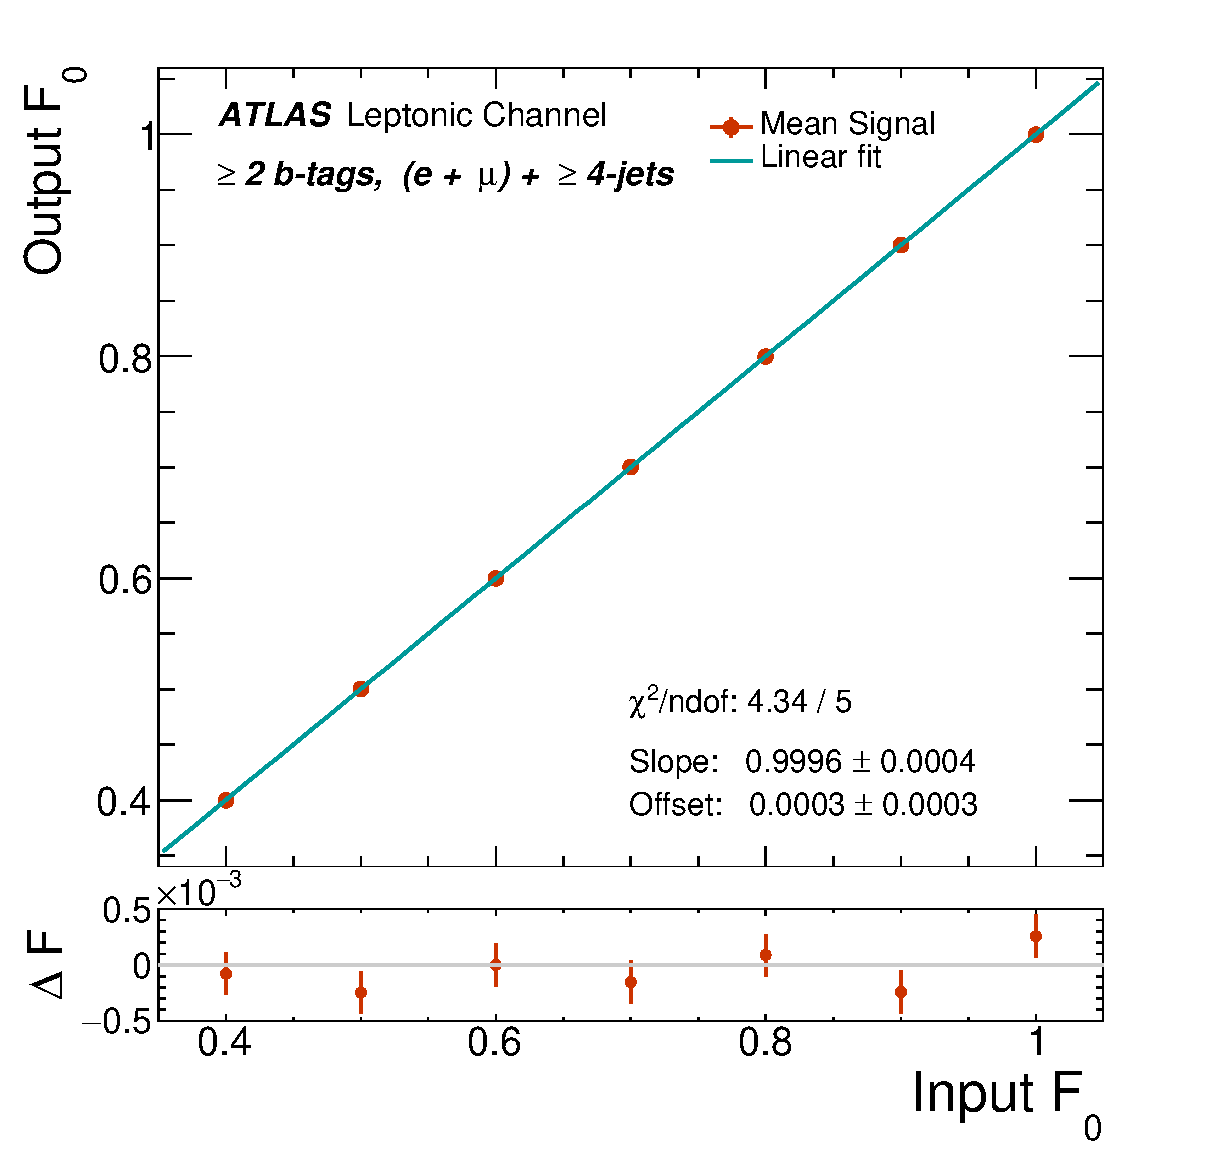
\includegraphics[height=50mm]{chapters/whel/figures/cali_curves_June-1-2017/Calicurve_F0_el_mu}
		\includegraphics[height=50mm]{chapters/whel/figures/cali_curves_June-1-2017/Calicurve_FL_el_mu}
		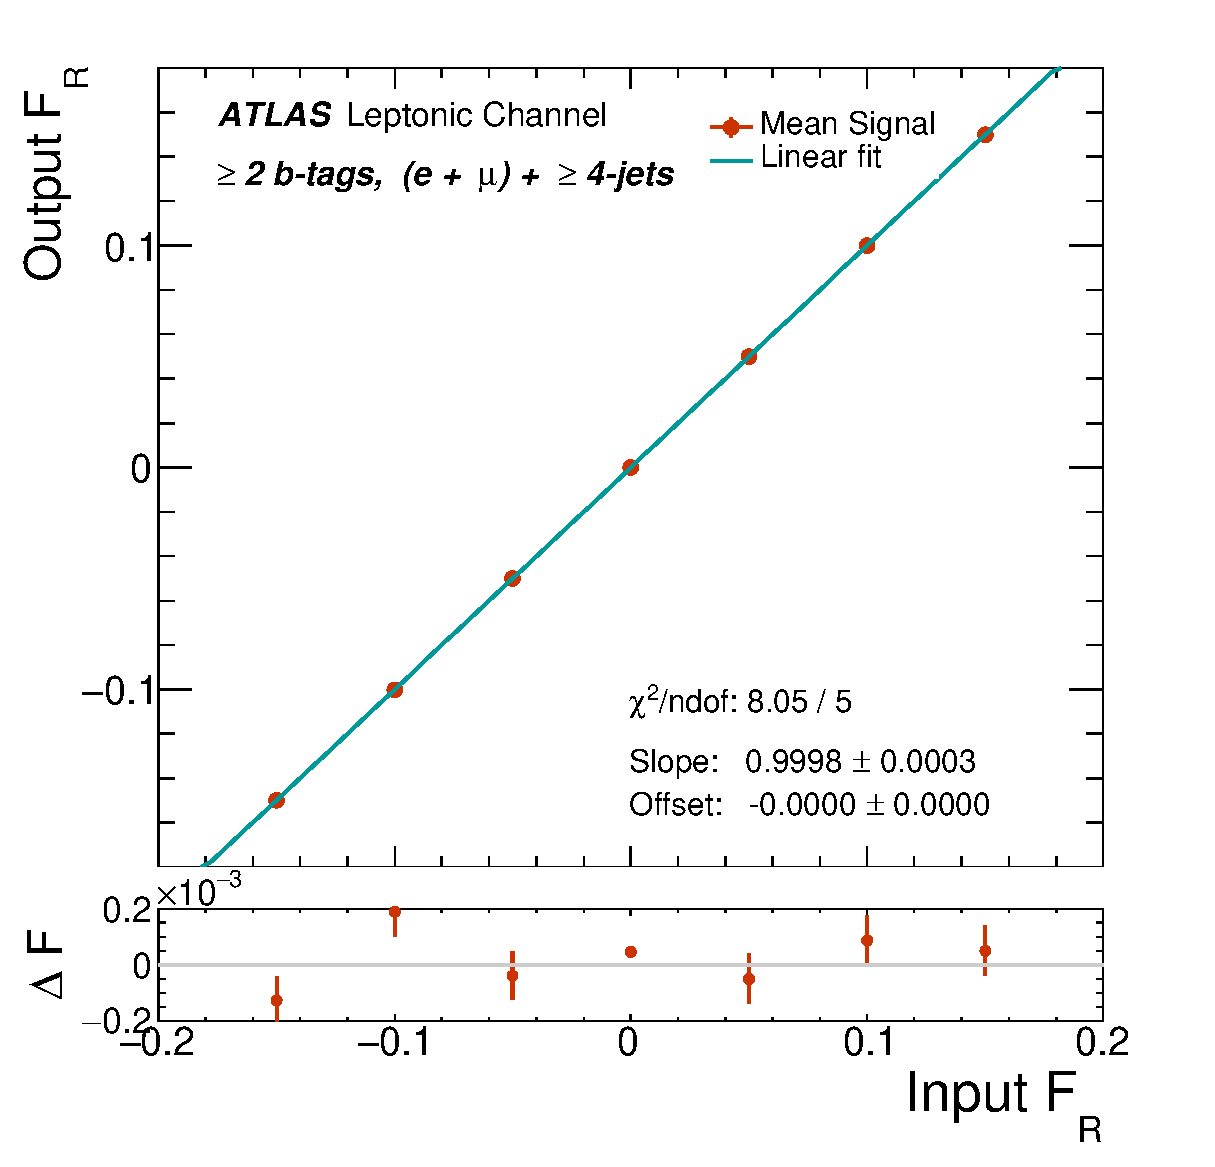
\includegraphics[height=50mm]{chapters/whel/figures/cali_curves_June-1-2017/Calicurve_FR_el_mu}
	\caption{Linearity checks for $F_{\text{0}}$, $F_{\text{L}}$, and $F_{\text{R}}$ in the electron+muon in two inclusive \bt tag region for the leptonic analyzer. 5000 sets of pseudo-data were fit to perform the test. Good closure is seen for all helicity fractions, and no bias is observed.}
	\label{fig:calibrationCurve_lephad}
\end{center}	
\end{figure}

\begin{comment}
The pull is defined as the difference between the fitted value of $N_{nom}$ and the value of $N_{j}$ used to create the pseudo-data which was fitted, divided by the uncertainty on $N_{j}$ of a fit:
\begin{equation}
\textrm{Pull}= \frac{N_{j} - N_{nom}}{\sigma_{N_{j}}}.
\label{eq:pull}
\end{equation}
For each value of $N_{nom}$ the pull distribution is obtained and the mean and RMS values are compared to the expectations of zero and unity respectively. No significant deviations from the expectations are observed. The complete set of pull distributions corresponding to the $\mu$+jets channel and templates of the hadronic angle for both \bt tag regions are presented in Appendix~\ref{app:fitCalibrations}.

\end{comment}
